% Options for packages loaded elsewhere
\PassOptionsToPackage{unicode}{hyperref}
\PassOptionsToPackage{hyphens}{url}
\PassOptionsToPackage{dvipsnames,svgnames,x11names}{xcolor}
%
\documentclass[
  12pt,
]{article}

\usepackage{amsmath,amssymb}
\usepackage{lmodern}
\usepackage{setspace}
\usepackage{iftex}
\ifPDFTeX
  \usepackage[T1]{fontenc}
  \usepackage[utf8]{inputenc}
  \usepackage{textcomp} % provide euro and other symbols
\else % if luatex or xetex
  \usepackage{unicode-math}
  \defaultfontfeatures{Scale=MatchLowercase}
  \defaultfontfeatures[\rmfamily]{Ligatures=TeX,Scale=1}
\fi
% Use upquote if available, for straight quotes in verbatim environments
\IfFileExists{upquote.sty}{\usepackage{upquote}}{}
\IfFileExists{microtype.sty}{% use microtype if available
  \usepackage[]{microtype}
  \UseMicrotypeSet[protrusion]{basicmath} % disable protrusion for tt fonts
}{}
\usepackage{xcolor}
\usepackage[margin=1in]{geometry}
\setlength{\emergencystretch}{3em} % prevent overfull lines
\setcounter{secnumdepth}{3}
% Make \paragraph and \subparagraph free-standing
\ifx\paragraph\undefined\else
  \let\oldparagraph\paragraph
  \renewcommand{\paragraph}[1]{\oldparagraph{#1}\mbox{}}
\fi
\ifx\subparagraph\undefined\else
  \let\oldsubparagraph\subparagraph
  \renewcommand{\subparagraph}[1]{\oldsubparagraph{#1}\mbox{}}
\fi


\providecommand{\tightlist}{%
  \setlength{\itemsep}{0pt}\setlength{\parskip}{0pt}}\usepackage{longtable,booktabs,array}
\usepackage{calc} % for calculating minipage widths
% Correct order of tables after \paragraph or \subparagraph
\usepackage{etoolbox}
\makeatletter
\patchcmd\longtable{\par}{\if@noskipsec\mbox{}\fi\par}{}{}
\makeatother
% Allow footnotes in longtable head/foot
\IfFileExists{footnotehyper.sty}{\usepackage{footnotehyper}}{\usepackage{footnote}}
\makesavenoteenv{longtable}
\usepackage{graphicx}
\makeatletter
\def\maxwidth{\ifdim\Gin@nat@width>\linewidth\linewidth\else\Gin@nat@width\fi}
\def\maxheight{\ifdim\Gin@nat@height>\textheight\textheight\else\Gin@nat@height\fi}
\makeatother
% Scale images if necessary, so that they will not overflow the page
% margins by default, and it is still possible to overwrite the defaults
% using explicit options in \includegraphics[width, height, ...]{}
\setkeys{Gin}{width=\maxwidth,height=\maxheight,keepaspectratio}
% Set default figure placement to htbp
\makeatletter
\def\fps@figure{htbp}
\makeatother
\newlength{\cslhangindent}
\setlength{\cslhangindent}{1.5em}
\newlength{\csllabelwidth}
\setlength{\csllabelwidth}{3em}
\newlength{\cslentryspacingunit} % times entry-spacing
\setlength{\cslentryspacingunit}{\parskip}
\newenvironment{CSLReferences}[2] % #1 hanging-ident, #2 entry spacing
 {% don't indent paragraphs
  \setlength{\parindent}{0pt}
  % turn on hanging indent if param 1 is 1
  \ifodd #1
  \let\oldpar\par
  \def\par{\hangindent=\cslhangindent\oldpar}
  \fi
  % set entry spacing
  \setlength{\parskip}{#2\cslentryspacingunit}
 }%
 {}
\usepackage{calc}
\newcommand{\CSLBlock}[1]{#1\hfill\break}
\newcommand{\CSLLeftMargin}[1]{\parbox[t]{\csllabelwidth}{#1}}
\newcommand{\CSLRightInline}[1]{\parbox[t]{\linewidth - \csllabelwidth}{#1}\break}
\newcommand{\CSLIndent}[1]{\hspace{\cslhangindent}#1}

\usepackage{fancyhdr}
\pagestyle{fancy}
\fancyhead{}
\fancyhead[R]{Profil cognitif des aphantasiques}
\renewcommand{\topfraction}{.85}
\renewcommand{\bottomfraction}{.7}
\renewcommand{\textfraction}{.15}
\renewcommand{\floatpagefraction}{.66}
\setcounter{topnumber}{3}
\setcounter{bottomnumber}{3}
\setcounter{totalnumber}{4}
\usepackage[font=footnotesize,labelfont=bf, textfont=it]{caption}
\usepackage{hyperref}
\usepackage[all]{nowidow}
\makeatletter
\makeatother
\makeatletter
\makeatother
\makeatletter
\@ifpackageloaded{caption}{}{\usepackage{caption}}
\AtBeginDocument{%
\ifdefined\contentsname
  \renewcommand*\contentsname{Table des matières}
\else
  \newcommand\contentsname{Table des matières}
\fi
\ifdefined\listfigurename
  \renewcommand*\listfigurename{Liste des Figures}
\else
  \newcommand\listfigurename{Liste des Figures}
\fi
\ifdefined\listtablename
  \renewcommand*\listtablename{Liste des Tables}
\else
  \newcommand\listtablename{Liste des Tables}
\fi
\ifdefined\figurename
  \renewcommand*\figurename{Figure}
\else
  \newcommand\figurename{Figure}
\fi
\ifdefined\tablename
  \renewcommand*\tablename{Table}
\else
  \newcommand\tablename{Table}
\fi
}
\@ifpackageloaded{float}{}{\usepackage{float}}
\floatstyle{ruled}
\@ifundefined{c@chapter}{\newfloat{codelisting}{h}{lop}}{\newfloat{codelisting}{h}{lop}[chapter]}
\floatname{codelisting}{Listing}
\newcommand*\listoflistings{\listof{codelisting}{Liste des Listings}}
\makeatother
\makeatletter
\@ifpackageloaded{caption}{}{\usepackage{caption}}
\@ifpackageloaded{subcaption}{}{\usepackage{subcaption}}
\makeatother
\makeatletter
\@ifpackageloaded{tcolorbox}{}{\usepackage[many]{tcolorbox}}
\makeatother
\makeatletter
\@ifundefined{shadecolor}{\definecolor{shadecolor}{rgb}{.97, .97, .97}}
\makeatother
\makeatletter
\makeatother
\ifLuaTeX
\usepackage[bidi=basic]{babel}
\else
\usepackage[bidi=default]{babel}
\fi
\babelprovide[main,import]{french}
% get rid of language-specific shorthands (see #6817):
\let\LanguageShortHands\languageshorthands
\def\languageshorthands#1{}
\ifLuaTeX
  \usepackage{selnolig}  % disable illegal ligatures
\fi
\IfFileExists{bookmark.sty}{\usepackage{bookmark}}{\usepackage{hyperref}}
\IfFileExists{xurl.sty}{\usepackage{xurl}}{} % add URL line breaks if available
\urlstyle{same} % disable monospaced font for URLs
% Make links footnotes instead of hotlinks:
\DeclareRobustCommand{\href}[2]{#2\footnote{\url{#1}}}
\hypersetup{
  pdflang={fr},
  colorlinks=true,
  linkcolor={blue},
  filecolor={Maroon},
  citecolor={Blue},
  urlcolor={Blue},
  pdfcreator={LaTeX via pandoc}}

\author{}
\date{}

\begin{document}
\begin{titlepage}
    \begin{center}
        \vspace*{1cm}

        \Huge
        Profil cognitif des aphantasiques :\\ étude exploratoire des stratégies de compensation spatiales et abstraites

        \vspace{0.5cm}
        \Large
        Simulation de données et analyses prévisionnelles\\ dans le cadre de l'UE Data Science
            
        \vfill
        \normalsize
        Maël Delem\\
        Colin Fourment\\
        Thomas Junoy\\
        Guillaume Leal de Almeida\\

            
        \vspace{0.8cm}
    
        
\includegraphics[width=0.4\textwidth]{./zd_logo/logo.png}
            
        13/02/2023
            
    \end{center}
\end{titlepage}

\newpage{}

\ifdefined\Shaded\renewenvironment{Shaded}{\begin{tcolorbox}[boxrule=0pt, frame hidden, interior hidden, breakable, sharp corners, borderline west={3pt}{0pt}{shadecolor}, enhanced]}{\end{tcolorbox}}\fi

\renewcommand*\contentsname{Table des matières}
{
\hypersetup{linkcolor=}
\setcounter{tocdepth}{3}
\tableofcontents
}
\setstretch{1.5}
\newpage

\hypertarget{introduction}{%
\section{Introduction}\label{introduction}}

\hypertarget{imagerie-visuelle-et-aphantasie}{%
\subsection{Imagerie visuelle et
aphantasie}\label{imagerie-visuelle-et-aphantasie}}

L'imagerie visuelle, parfois désignée poétiquement comme le fait de
``voir dans les yeux de l'esprit'', désigne l'expérience visuelle
quasi-perceptive d'images mentales en l'absence du stimulus externe
correspondant
(\protect\hyperlink{ref-monzelAphantasiaDysikonesiaAnauralia2022}{Monzel
et al., 2022};
\protect\hyperlink{ref-pearsonHumanImaginationCognitive2019}{Pearson,
2019}). L'imagerie visuelle est considérée par la plupart des gens comme
un élément central de leur vie mentale quotidienne, dans la mémorisation
et la récupération d'informations sur des lieux, des objets ou des
personnes connus, dans le vagabondage mental et la rêverie, voire plus
généralement dans la créativité
(\protect\hyperlink{ref-zemanLivesImageryCongenital2015}{A. Zeman et
al., 2015}). Il a été démontré qu'elle joue un rôle prépondérant dans de
nombreux processus cognitifs, tels que la mémoire autobiographique, la
mémoire épisodique et la prospection d'évènements futurs
(\protect\hyperlink{ref-greenbergRoleVisualImagery2014}{Greenberg \&
Knowlton, 2014}), la mémoire de travail visuelle
(\protect\hyperlink{ref-pearsonHumanImaginationCognitive2019}{Pearson,
2019}).

Cependant, il a été démontré qu'il pouvait exister une grande
variabilité interindividuelle dans l'imagerie visuelle, et que certaines
personnes pouvaient même en être totalement dépourvues. L'une des toutes
premières études sur l'imagerie visuelle, une enquête menée par Sir
Francis Galton en 1880, a apporté les premiers témoignages de la grande
variété de la capacité des gens à produire des images mentales. Son
``enquête sur la table du petit-déjeuner'' invitait les participants à
visualiser leur table du matin et à évaluer ``l'illumination, la
définition et la coloration'' des images mentales qu'ils en avaient. À
son grand étonnement, il a découvert que certaines personnes
interrogées, parmi lesquelles beaucoup de ses collègues, dans ses termes
des ``hommes de science'', ont protesté que l'imagerie mentale leur
était inconnue - tout comme les daltoniens ne pouvaient pas concevoir la
nature de la couleur, ces personnes ne pouvaient pas concevoir la nature
de l'imagerie mentale
(\protect\hyperlink{ref-galtonSTATISTICSMENTALIMAGERY1880}{Galton,
1880}).

Il est intéressant de noter que, bien qu'il y ait eu une résurgence des
recherches et des débats sur l'imagerie mentale à la fin du siècle qui a
suivi (e.g. Kosslyn et al.
(\protect\hyperlink{ref-kosslynCognitiveNeuroscienceMental1995}{1995});
Pylyshyn
(\protect\hyperlink{ref-pylyshynMentalImagerySearch2002}{2002});
Reisberg et al.
(\protect\hyperlink{ref-reisbergIntuitionsIntrospectionsImagery2002}{2002})),
cette condition d'``imagination aveugle'' n'a pas suscité beaucoup
d'attention. Une exception notable est Faw
(\protect\hyperlink{ref-fawConflictingIntuitionsMay2009}{2009}), qui a
soulevé le fait que les théories des chercheurs sur l'imagerie
pourraient être fortement biaisées par leur propre expérience subjective
de celle-ci. Il a indiqué que les ``non-visualiseurs'', ignorés par la
recherche jusqu'à présent, pourraient représenter 2 à 3 \% des
personnes, selon son enquête (\emph{N} = 2500). En 2010, Zeman et
al.~ont rapporté le cas d'un patient qui a perdu la capacité de produire
des images mentales après avoir subi une intervention chirurgicale
(\protect\hyperlink{ref-zemanLossImageryPhenomenology2010}{A. Z. J.
Zeman et al., 2010}). L'article a attiré l'attention du public après un
reportage dans le magazine \emph{Discovery}
(\protect\hyperlink{ref-zimmerBrainLookDeep2010}{Zimmer, 2010}) : bien
qu'il s'agisse apparemment d'imagination aveugle ``acquise'', l'article
a conduit de nombreuses personnes à se reconnaître dans cette condition
et à contacter l'équipe pour témoigner de leur expérience, avec la
différence importante qu'elles avaient toujours eu cette absence
d'imagerie. En décrivant leurs cas, Zeman et al.
(\protect\hyperlink{ref-zemanLivesImageryCongenital2015}{2015}) ont créé
le terme ``\emph{aphantasie}'' pour décrire l'absence d'imagerie
mentale.

L'aphantasie, en tant que terme et phénomène, a attiré l'attention des
médias et a entraîné une augmentation importante du nombre de personnes
signalant leur cas d'imagerie extrême
(\protect\hyperlink{ref-monzelAphantasiaDysikonesiaAnauralia2022}{Monzel
et al., 2022}). Les études à grande échelle sur les extrêmes de
l'imagerie visuelle suggèrent une prévalence de 2-4\% d'aphantasie dans
la population générale (C. J. Dance et al.
(\protect\hyperlink{ref-dancePrevalenceAphantasiaImagery2022}{2022}) :
\emph{N} = 1004 ; A. J. Dawes et al.
(\protect\hyperlink{ref-dawesCognitiveProfileMultisensory2020}{2020}) :
\emph{N} = 715 ; Faw
(\protect\hyperlink{ref-fawConflictingIntuitionsMay2009}{2009}) :
\emph{N} = 2500 ; Palermo et al.
(\protect\hyperlink{ref-palermoCongenitalLackExtraordinary2022}{2022}) :
\emph{N} = 490 ; Takahashi et al.
(\protect\hyperlink{ref-takahashiDiversityAphantasiaRevealed2022}{2022}):
\emph{N} = 2885 ; A. Zeman et al.
(\protect\hyperlink{ref-zemanPhantasiaPsychologicalSignificance2020}{2020}))
avec de nombreuses variations (entre 0,5 et 11\%) selon les seuils
choisis pour caractériser l'affection. L'étude de l'aphantasie est
récente, et bien qu'il n'existe pas actuellement de '' profil ''
clairement défini des individus aphantasiques, la recherche a lentement
assemblé plusieurs caractéristiques associées à cette condition.

\hypertarget{les-corruxe9lats-de-laphantasie}{%
\subsection{Les corrélats de
l'aphantasie}\label{les-corruxe9lats-de-laphantasie}}

Depuis 2015, le nouveau champ scientifique de l'aphantasie a construit
un corpus de divers corrélats cognitifs, comportementaux et
physiologiques de l'aphantasie. Communément, l'aphantasie est évaluée
dans des études à grande échelle en utilisant des auto-rapports
qualitatifs et le questionnaire Vividness of Visual Imagery
(\protect\hyperlink{ref-marksVividnessVisualImagery1973}{Marks, 1973}),
même si le seuil VVIQ choisi pour caractériser les personnes ayant une
faible imagerie varie selon les études (entre 16 \textasciitilde{} 30).
En utilisant les questionnaires comme point de départ, plusieurs études
expérimentales ont été en mesure de corréler une faible imagerie
visuelle avec des caractéristiques distinctes.

\hypertarget{corruxe9lats-cognitifs}{%
\subsubsection{Corrélats cognitifs}\label{corruxe9lats-cognitifs}}

La plupart des études à grande échelle existantes sur l'aphantasie ont
porté sur les capacités de mémoire des aphantasiques, et ont montré des
corrélations entre leur faible imagerie et des déficiences en mémoire
autobiographique et épisodique
(\protect\hyperlink{ref-dawesCognitiveProfileMultisensory2020}{A. J.
Dawes et al., 2020};
\protect\hyperlink{ref-miltonBehavioralNeuralSignatures2021}{Milton et
al., 2021};
\protect\hyperlink{ref-zemanPhantasiaPsychologicalSignificance2020}{A.
Zeman et al., 2020}). Les aphantasiques, lorsqu'on leur demande
d'évaluer leur mémoire autobiographique, l'évaluent le plus souvent plus
bas que les témoins
(\protect\hyperlink{ref-zemanPhantasiaPsychologicalSignificance2020}{A.
Zeman et al., 2020},
\protect\hyperlink{ref-zemanLivesImageryCongenital2015}{2015}). L'un de
ces rapports subjectifs a fait émerger la possibilité d'une association
de l'aphantasie avec les syndromes de mémoire autobiographique
sévèrement déficiente
(\protect\hyperlink{ref-watkinsPhantasiaSeverelyDeficient2018}{Watkins,
2018}). En accord avec les auto-rapports et les données
neuropsychologiques sur la mémoire épisodique, Dawes et al.
(\protect\hyperlink{ref-dawesInnerVisionsMind2022}{2022}) ont démontré,
à l'aide de l'Autobiographical Interview, une mesure comportementale de
la spécificité et de la richesse des détails épisodiques (combinant donc
des évaluations subjectives et objectives) que l'aphantasie était
également associée à une réduction des détails épisodiques pour les
évènements passés et futurs. Leurs résultats sont également en accord
avec ceux de Milton et al.
(\protect\hyperlink{ref-miltonBehavioralNeuralSignatures2021}{2021}) qui
ont mis en évidence une réduction de l'``imagination'' temporelle et
atemporelle, à savoir la capacité à simuler des évènements fictifs.
L'aphantasie a également été associée à la prosopagnosie - la difficulté
à reconnaître les visages
(\protect\hyperlink{ref-dawesCognitiveProfileMultisensory2020}{A. J.
Dawes et al., 2020};
\protect\hyperlink{ref-miltonBehavioralNeuralSignatures2021}{Milton et
al., 2021};
\protect\hyperlink{ref-palermoCongenitalLackExtraordinary2022}{Palermo
et al., 2022};
\protect\hyperlink{ref-zemanPhantasiaPsychologicalSignificance2020}{A.
Zeman et al., 2020}), et à des rêves nocturnes et diurnes
qualitativement appauvris
(\protect\hyperlink{ref-dawesCognitiveProfileMultisensory2020}{A. J.
Dawes et al., 2020};
\protect\hyperlink{ref-zemanPhantasiaPsychologicalSignificance2020}{A.
Zeman et al., 2020}).

\hypertarget{corruxe9lats-comportementaux-et-physiologiques}{%
\subsubsection{Corrélats comportementaux et
physiologiques}\label{corruxe9lats-comportementaux-et-physiologiques}}

Comme nous l'avons mentionné, la plupart des études sur l'aphantasie se
sont appuyées sur des évaluations subjectives, des questionnaires et des
rapports personnels pour identifier et évaluer la condition et
l'imagerie visuelle. Bien que les phénomènes subjectifs rapportés par
les aphantasiques montrent une cohérence remarquable, les rapports à la
première personne et l'introspection restent faillibles
(\protect\hyperlink{ref-miltonBehavioralNeuralSignatures2021}{Milton et
al., 2021};
\protect\hyperlink{ref-zemanPhantasiaPsychologicalSignificance2020}{A.
Zeman et al., 2020}). Les différences dans les jugements d'imagerie
visuelle pourraient être liées à une mauvaise métacognition, résultant
en une incapacité des aphantasiques à percevoir consciemment leur
imagerie potentiellement effective. Pour surmonter cette limitation, de
nouvelles méthodes de mesure de l'imagerie visuelle et de son absence
ont été développées afin de trianguler ces auto-rapports subjectifs avec
des marqueurs comportementaux et physiologiques objectifs. Ainsi, il a
été démontré que les personnes atteintes d'aphantasie ne présentent pas
d'amorçage par l'imagerie visuelle par rapport aux témoins en utilisant
le paradigme de rivalité binoculaire basé sur les sens
(\protect\hyperlink{ref-keoghBlindMindNo2018}{Keogh \& Pearson, 2018},
\protect\hyperlink{ref-keoghAttentionDrivenPhantom2020}{2020}) ; elles
se souviennent de moins d'objets et de couleurs que les témoins à partir
de scènes étudiées
(\protect\hyperlink{ref-bainbridgeQuantifyingAphantasiaDrawing2021}{Bainbridge
et al., 2021}) ; ils ont montré moins de sensibilité sensorielle dans
une tâche d'éblouissement de motifs visuels, ce qui suggère que
l'imagerie sensorielle et la sensibilité sensorielle sont liées
(\protect\hyperlink{ref-danceLessSensoryOverwhelm2022}{C. Dance, 2022};
\protect\hyperlink{ref-danceWhatLinkMental2021}{C. J. Dance et al.,
2021}) ; ils n'ont pas montré de réponse de conductivité cutanée à
l'imagerie émotionnelle lors de la lecture de scénarios effrayants
(Wicken et al., 2019) ; et enfin, ils n'ont pas montré de réponse
pupillaire à des formes claires ou sombres imaginées
(\protect\hyperlink{ref-lachlanPupillaryLightResponse2022}{Lachlan et
al., 2022}). Ces deux derniers paradigmes en particulier ont établi les
premiers indices physiologiques de la force de l'imagerie sensorielle et
phénoménologique, et les premières validations physiologiques de
l'aphantasie. L'investigation du phénomène de l'imagerie visuelle par
ces méthodes objectives a permis de rassembler des preuves solides en
faveur de la conception de l'aphantasie comme une véritable absence (ou
une réduction sévère) de l'imagerie visuelle plutôt que comme un déficit
métacognitif.

\hypertarget{laphantasie-est-elle-un-trouble}{%
\subsubsection{L'aphantasie est elle un trouble
?}\label{laphantasie-est-elle-un-trouble}}

L'aphantasie a été associée dans la littérature récente à une série de
déficiences et de déficits, et est donc souvent logiquement désignée
comme un handicap ou un trouble (e.g. Blomkvist
(\protect\hyperlink{ref-blomkvistAphantasiaSearchTheory2022}{2022});
Fox-Muraton
(\protect\hyperlink{ref-fox-muratonWorldImaginationConsequences2021}{2021}))
; certaines revues vont jusqu'à caractériser la condition comme un
ensemble de déficiences résultant d'un dysfonctionnement d'un système
cognitif
(\protect\hyperlink{ref-blomkvistAphantasiaSearchTheory2022}{Blomkvist,
2022}). Bien que ce point de vue puisse être justifié d'une certaine
manière si l'on considère que les déficiences de l'imagerie mentale
peuvent survenir à la suite de lésions cérébrales, d'opérations
chirurgicales ou de troubles psychiatriques - une condition appelée
``aphantasie acquise''
(\protect\hyperlink{ref-bartolomeoAssessingCausalRole2020}{Bartolomeo et
al., 2020};
\protect\hyperlink{ref-cavedon-taylorPredictiveProcessingPerception2021}{Cavedon-Taylor,
2021}; \protect\hyperlink{ref-farahCaseStudyMental1988}{Farah et al.,
1988}; \protect\hyperlink{ref-spagnaChapterVisualMental2022}{Spagna,
2022}; \protect\hyperlink{ref-zagoCharcotBernardCase2011}{Zago et al.,
2011}; \protect\hyperlink{ref-zemanLossImageryPhenomenology2010}{A. Z.
J. Zeman et al., 2010}), on peut trouver à redire sur plusieurs
observations dans l'aphantasie congénitale (c'est-à-dire à vie). Des
preuves empiriques provenant de plusieurs études soulignent que les
aphantasiques pourraient n'avoir aucune différence de performance dans
divers types de tâches présumées nécessiter une imagerie visuelle.

Tout d'abord, en contraste frappant avec les résultats suggestifs sur la
mémoire épisodique, les aphantasiques ont des performances aussi
précises que les témoins dans plusieurs paradigmes de mémoire de travail
visuelle en laboratoire et en clinique
(\protect\hyperlink{ref-keoghVisualWorkingMemory2021}{Keogh et al.,
2021}; \protect\hyperlink{ref-knightMemoryImageryNo2022}{Knight et al.,
2022}) ; ils ont également les mêmes performances dans les tâches de
mémoire clinique évaluant le rappel antérograde
(\protect\hyperlink{ref-miltonBehavioralNeuralSignatures2021}{Milton et
al., 2021}) et la mémoire de reconnaissance pour le matériel verbal et
visuel
(\protect\hyperlink{ref-bainbridgeQuantifyingAphantasiaDrawing2021}{Bainbridge
et al., 2021};
\protect\hyperlink{ref-miltonBehavioralNeuralSignatures2021}{Milton et
al., 2021}) ; ils ne présentent pas de différences significatives dans
les tâches de mémoire sémantique
(\protect\hyperlink{ref-dawesCognitiveProfileMultisensory2020}{A. J.
Dawes et al., 2020};
\protect\hyperlink{ref-miltonBehavioralNeuralSignatures2021}{Milton et
al., 2021}) ; de même, ils ne présentent pas de déficience de la mémoire
déclarative générale ou visuelle dans une batterie de tests
neuropsychologiques
(\protect\hyperlink{ref-pounderOnlyMinimalDifferences2022}{Pounder et
al., 2022}). Keogh et al.
(\protect\hyperlink{ref-keoghVisualWorkingMemory2021}{2021}) soulignent
également dans leur étude le fait que les performances des aphantasiques
dans les tâches d'imagerie visuelle peuvent s'appuyer sur des stratégies
différentes, sur la base des différences notables entre leurs stratégies
rapportées, et corroborées par une absence d'effet d'orientation dans
leurs réponses, supposé se produire en raison du recrutement sensoriel.
Zeman et al.
(\protect\hyperlink{ref-zemanPhantasiaPsychologicalSignificance2020}{2020})
font état de rapport similaires d'aphantasiques utilisant des stratégies
alternatives\footnote{Il est à noter que l'utilisation de la
  terminologie ``\emph{stratégie alternative}'' et
  ``\emph{compensation}'' vient du fait de la majorité des personnes
  ``non-aphantasiques'' : elle souligne aussi la difficulté pour
  quelqu'un disposant d'imagerie visuelle à ne pas voir son absence
  comme un trouble.} pour résoudre une tâche de comptage du nombre de
fenêtres chez soi : ils expliquaient avoir recours à l'imagerie
spatiale, à l'imagerie kinesthésique (i.e.~de mouvement), et aux
connaissances amodales.

Pris ensemble, ces résultats suggèrent que les aphantasiques ne
présentent pas de problèmes de mémoire de travail, de reconnaissance ou
de mémoire déclarative (générale ou visuelle) qui pourraient s'avérer
affecter leur vie quotidienne. Ils reflètent également le fait que ces
performances pourraient s'appuyer sur des stratégies alternatives non
visuelles tout aussi adaptées pour résoudre des problèmes supposés
auparavant nécessiter une imagerie visuelle. Ceci plaide pour considérer
que les aphantasiques utilisent des approches alternatives qui
pourraient ne pas être uniquement de la compensation, mais un tout autre
'' mode de fonctionnement humain du traitement de l'information ''
(\protect\hyperlink{ref-zemanPhantasiaPsychologicalSignificance2020}{A.
Zeman et al., 2020}) : si nous adhérons à ce point de vue, les
spécificités des différences entre ces modes restent encore à
déterminer.

\hypertarget{expuxe9riences-de-vie-et-styles-cognitifs}{%
\subsubsection{Expériences de vie et ``styles
cognitifs''}\label{expuxe9riences-de-vie-et-styles-cognitifs}}

En accord avec le fait que leur vie quotidienne ne semble pas être
affectée par leur état, les aphantasiques sont le plus souvent
inconscients de leur celui-ci, qui est de la même manière invisible pour
les gens, puisqu'ils ne vivent apparemment pas différemment de n'importe
qui d'autre
(\protect\hyperlink{ref-kendleAphantasiaExperiencesPerceptions2017}{Kendle,
2017}; \protect\hyperlink{ref-zemanLivesImageryCongenital2015}{A. Zeman
et al., 2015}). Bien qu'il n'existe pas, à ce jour, d'étude systématique
du profil démographique des aphantasiques, les résultats préliminaires
d'une étude récente
(\protect\hyperlink{ref-zemanPhantasiaPsychologicalSignificance2020}{A.
Zeman et al., 2020}) apportent un éclairage sur les préférences
professionnelles potentielles des personnes dotées d'imageries extrêmes.
En effet, les données des questionnaires de milliers de participants sur
l'imagerie visuelle ont révélé que les extrêmes de ce spectre
présentaient des associations comportementales et psychologiques
distinctes, y compris des préférences professionnelles : alors que les
personnes présentant une imagerie visuelle extrêmement élevée (appelées
``hyperphantasiques'') avaient tendance à travailler dans des
professions traditionnellement considérées comme ``créatives'' (à savoir
les arts, le design, le divertissement et la communication), les
aphantasiques étaient plus susceptibles de travailler dans
l'informatique, les mathématiques et les sciences
(\protect\hyperlink{ref-crowderDifferencesSpatialVisualization2018}{Crowder,
2018};
\protect\hyperlink{ref-zemanPhantasiaPsychologicalSignificance2020}{A.
Zeman et al., 2020}). Ces résultats apportent un autre argument, d'un
point de vue comportemental plus large, vers l'idée d'une tension entre
deux ``styles cognitifs''
(\protect\hyperlink{ref-kozhevnikovSpatialObjectVisualizers2005}{Kozhevnikov
et al., 2005}), et une vision de l'aphantasie et de l'hyperphantasie
comme des conditions équilibrées, avec des avantages et des
inconvénients
(\protect\hyperlink{ref-zemanPhantasiaPsychologicalSignificance2020}{A.
Zeman et al., 2020}).

Bien que les affirmations initiales de Galton selon lesquelles les
``hommes de science'' manquaient d'imagerie mentale aient été contestées
depuis - et qu'il ait été démontré qu'il s'agissait d'une généralisation
excessive de son observation de quelques répondants particulièrement
inhabituels parmi ses collègues scientifiques
(\protect\hyperlink{ref-brewerScientistsAreNot2006}{Brewer \&
Schommer-Aikins, 2006}) - son récit reste intéressant en suivant
l'inférence inverse : Si les aphantasiques sont effectivement très peu
nombreux, comme l'ont montré des données plus récentes, ont-ils vraiment
tendance à se tourner vers les domaines scientifiques ? Les premiers
résultats concernant les aphantasiques semblent corroborer cette
intuition. Pourtant, quelles bases cognitives pourraient sous-tendre ces
différentes stratégies mentales des aphantasiques et ces apparentes
affinités intellectuelles ? Quelle est la nature des différents
``modes'' supposés de traitement de l'information visuelle ?

\hypertarget{stratuxe9gies-et-muxe9canismes-de-compensation-possibles-dans-laphantasie}{%
\subsection{Stratégies et mécanismes de compensation possibles dans
l'aphantasie}\label{stratuxe9gies-et-muxe9canismes-de-compensation-possibles-dans-laphantasie}}

\hypertarget{opposition-entre-le-visuel-et-labstrait}{%
\subsubsection{Opposition entre le visuel et
l'abstrait}\label{opposition-entre-le-visuel-et-labstrait}}

Galton expliquait son hypothèse sur les scientifiques par le potentiel
antagonisme entre la visualisation d'images mentales et la pensée
abstraite et holistique. Il constatait cependant que ses collègues
aphantasiques\footnote{L'appellation est anachronique mais utilisée à
  des fins de clarté.} pouvaient tout de même donner des descriptions
précises de scènes visuelles. Il formulait déjà l'hypothèse d'une
compensation par d'autres modes de conception, notamment des modes de
pensées liés à l'imagerie motrice (la représentation mentale du
mouvement et de la sensation de bouger)
(\protect\hyperlink{ref-galtonSTATISTICSMENTALIMAGERY1880}{Galton,
1880}). Dans des études sur le raisonnement et la visualisation mentale,
Knauff et Johnson-Laird
(\protect\hyperlink{ref-knauffVisualImageryCan2002}{2002}) ont montré
que l'imagerie visuelle pouvait ralentir le processus de raisonnement,
contrairement à l'imagerie visuospatiale, spatiale ou à la
conceptualisation amodale.

\hypertarget{stratuxe9gies-verbales-suxe9mantiques-et-abstraites}{%
\subsubsection{Stratégies verbales, sémantiques et
abstraites}\label{stratuxe9gies-verbales-suxe9mantiques-et-abstraites}}

Zeman élabore aussi sur la compensation en émettant des hypothèses sur
le développement de stratégies alternatives par les domaines verbaux,
abstraits ou logiques, et pointe vers l'idée d'un traitement de
l'information préférentiellement sémantique et factuel chez les
aphantasiques
(\protect\hyperlink{ref-zemanPhantasiaPsychologicalSignificance2020}{A.
Zeman et al., 2020},
\protect\hyperlink{ref-zemanLivesImageryCongenital2015}{2015}). Junichi
et Jiro
(\protect\hyperlink{ref-junichiPreliminarySinglecaseStudy2020}{2020})
ont étudié le cas d'un aphantasique par des questionnaires
d'auto-évaluation. Le participant présentait des capacités d'imagerie
auditive préservées et rapportait avoir recours à des stratégies
verbales en réponse à des situations supposées comme nécessitant de
l'imagerie visuelle, corroborant les observations de Zeman et al
(\protect\hyperlink{ref-zemanPhantasiaPsychologicalSignificance2020}{2020}).
Ganczarek et al.
(\protect\hyperlink{ref-ganczarekRememberThingsCan2020}{2020}) ont
étudié le cas d'une aphantasique présentant des résultats faibles à la
composante ``imagerie visuelle-objet'' (correspondant à ce qui est
couramment appelé ``imagerie visuelle'') du questionnaire OSIVQ, mais
des scores spatiaux et verbaux dans la norme, témoignant d'une
préférence pour le raisonnement spatial et verbal. Elle ne présentait
pas de troubles de la mémoire de travail visuospatiale. Son QI total
était élevé (128), avec une différence marquée entre le QI verbal et le
QI performance au profit du verbal (138 et 114). Milton et al.
(\protect\hyperlink{ref-miltonBehavioralNeuralSignatures2021}{2021})
soulignent aussi ce résultat dans leur étude, les participants
aphantasiques présentant un QI plus élevé que les participants
hyperphantasiques. Une hypothèse liée aux fonctionnements alternatifs
pourrait concerner les fonctions exécutives, notamment la flexibilité
mentale (capacité de passer d'une tâche cognitive à une autre) : les
aphantasiques devant utiliser un plus grand panel de stratégies pour
traiter des tâches mentales visuelles, ils pourraient donc présenter des
fonctions exécutives de plus haut niveau que la moyenne.\\
Suggate et Lenhard
(\protect\hyperlink{ref-suggateMentalImagerySkill2022}{2022}) ont montré
qu'une mesure objective de l'imagerie mentale (l'\emph{Imagery
Comparison Task}) était un prédicteur significatif des performances de
compréhension en lecture, alors que les auto-évaluations subjectives (le
\emph{Plymouth Sensory Imagery Questionnaire} et le \emph{Spontaneous
Use of Imagery Survey}) ne montraient pas de lien. Ces résultats
montrent donc pour la première fois que les processus d'imagerie mentale
sont intrinsèquement liés aux performances en lecture. Cette étude
souligne aussi l'intérêt de l'utilisation d'une tâche écologique
impliquant les images mentales par rapport aux traditionnels
questionnaires.

\hypertarget{imagerie-visuelle-objet-et-visuospatiale}{%
\subsubsection{Imagerie visuelle-objet et
visuospatiale}\label{imagerie-visuelle-objet-et-visuospatiale}}

Autre hypothèse reposerait sur la distinction fondamentale dans
l'imagerie visuelle entre deux composantes, l'imagerie
\emph{visuelle-objet} (c'est-à-dire la représentation mentale des
caractéristiques visuelles d'un objet telles que la forme, la luminosité
ou la couleur) et l'imagerie \emph{visuelle-spatiale} (ou visuospatiale
- i.e.~la représentation mentale des emplacements spatiaux et des
relations entre les parties d'un objet). Un résultat expérimental
cohérent dans toutes les études récentes sur l'aphantasie est l'imagerie
spatiale préservée des aphantasiques, par opposition à leur imagerie
d'objet altérée. En utilisant l'OSIQ, plusieurs études ont montré qu'il
n'y avait pas de différence significative entre les aphantasiques et les
témoins sur les items d'imagerie spatiale
(\protect\hyperlink{ref-bainbridgeQuantifyingAphantasiaDrawing2021}{Bainbridge
et al., 2021};
\protect\hyperlink{ref-dawesCognitiveProfileMultisensory2020}{A. J.
Dawes et al., 2020}; \protect\hyperlink{ref-keoghBlindMindNo2018}{Keogh
\& Pearson, 2018};
\protect\hyperlink{ref-miltonBehavioralNeuralSignatures2021}{Milton et
al., 2021};
\protect\hyperlink{ref-zemanPhantasiaPsychologicalSignificance2020}{A.
Zeman et al., 2020}). Les aphantasiques ont obtenu des résultats précis
au test des mannequins et aux tâches de rotation mentale, impliquant la
rotation mentale d'avatars ou d'objets
(\protect\hyperlink{ref-crowderDifferencesSpatialVisualization2018}{Crowder,
2018};
\protect\hyperlink{ref-miltonBehavioralNeuralSignatures2021}{Milton et
al., 2021};
\protect\hyperlink{ref-pounderOnlyMinimalDifferences2022}{Pounder et
al., 2022}) - bien que Pounder et al.
(\protect\hyperlink{ref-pounderOnlyMinimalDifferences2022}{2022}) aient
signalé des temps de réponse plus lents pour les aphantasiques à très
faible imagerie. Dans la même lignée, Bainbridge et al.
(\protect\hyperlink{ref-bainbridgeQuantifyingAphantasiaDrawing2021}{2021})
ont observé que, lorsqu'on leur demande de dessiner de mémoire une scène
vue précédemment, les aphantasiques se souviennent de beaucoup moins
d'objets et de façon moins détaillée que les témoins, mais avec des
tailles, des emplacements et une organisation corrects, voire plus
précis. Ensemble, ces résultats suggèrent que les ``aphantasiques''
actuellement les plus étudiés sont en fait des \emph{aphantasiques
``objets''}, avec une imagerie visuospatiale intacte.

Des résultats intéressants dans la littérature sur l'imagerie spatiale
semblent faire écho aux premiers résultats de Zeman et al.
(\protect\hyperlink{ref-zemanPhantasiaPsychologicalSignificance2020}{2020})
sur les préférences professionnelles des aphantasiques (objet). Les
hautes performances dans les tests de visualisation spatiale sont
corrélées aux performances professionnelles et académiques dans divers
domaines des STEM (\emph{Science, Technology, Engineering and
Mathematics}), notamment la physique, la chimie organique, la géologie,
les mathématiques, ainsi que la chirurgie, l'architecture et le
raisonnement mécanique
(\protect\hyperlink{ref-colemanSpatialPerceptionSkills1998}{Coleman \&
Gotch, 1998};
\protect\hyperlink{ref-hegartyIndividualDifferencesSpatial2005}{Hegarty
\& Waller, 2005};
\protect\hyperlink{ref-keehnerSpatialAbilityExperience2004}{Keehner et
al., 2004};
\protect\hyperlink{ref-kozhevnikovSpatialVisualizationPhysics2007}{Kozhevnikov
et al., 2007};
\protect\hyperlink{ref-orionRelationshipEarthScienceEducation1997}{Orion
et al., 1997}; \protect\hyperlink{ref-waiSpatialAbilitySTEM2009}{Wai et
al., 2009}). D'autres études ont mis en évidence que la réussite dans
les STEM reposait sur des capacités fondamentales d'imagerie spatiale
telles que l'imagination de structures schématiques ou l'exécution de
transformations spatiales mentales
(\protect\hyperlink{ref-kozhevnikovSpatialVisualizationPhysics2007}{Kozhevnikov
et al., 2007}; \protect\hyperlink{ref-waiSpatialAbilitySTEM2009}{Wai et
al., 2009}). Ces considérations jettent également un nouvel éclairage
sur les observations et les intuitions de Galton
(\protect\hyperlink{ref-galtonSTATISTICSMENTALIMAGERY1880}{1880})
concernant les scientifiques. Blajenkova et al.
(\protect\hyperlink{ref-blajenkovaObjectSpatialImagery2006}{Blajenkova
et al., 2006a}) ont proposé une explication avec le clivage
objet-spatial : les scientifiques ne seraient pas complètement
déficients en imagerie visuelle générale, comme le suggérait Galton,
mais seraient seulement sélectivement déficients en imagerie
visuelle-objet.

En outre, les recherches sur les différences individuelles en matière
d'imagerie ont démontré que les scientifiques et les ingénieurs ont
tendance à être des imageurs spatiaux tandis que les artistes visuels
ont tendance à être des imageurs objet
(\protect\hyperlink{ref-blajenkovaObjectSpatialImagery2006}{Blajenkova
et al., 2006a};
\protect\hyperlink{ref-blazhenkovaVisualobjectAbilityNew2010}{Blazhenkova
\& Kozhevnikov, 2010},
\protect\hyperlink{ref-blazhenkovaNewObjectspatialverbalCognitive2009}{2009};
\protect\hyperlink{ref-kozhevnikovTradeoffObjectSpatial2010}{Kozhevnikov
et al., 2010};
\protect\hyperlink{ref-kozhevnikovSpatialObjectVisualizers2005}{Kozhevnikov
et al., 2005}). Ces études ont non seulement montré, par le biais de
rapports subjectifs, que les artistes et les scientifiques différaient
en termes d'imagerie, mais elles ont également mis en évidence des
différences de performance : les artistes ont obtenu de meilleurs
résultats dans les tâches nécessitant la visualisation d'objets (par
exemple, la création de représentations d'images et de couleurs,
l'identification d'objets dégradés) ; tandis que les visualiseurs
spatiaux et les scientifiques ont obtenu de meilleurs résultats dans les
tâches nécessitant une visualisation spatiale (par exemple, la rotation
mentale, le pliage de papier, la recherche d'un emplacement). Enfin,
Kozhevnikov et al.
(\protect\hyperlink{ref-kozhevnikovCreativityVisualizationAbilities2013}{Kozhevnikov
et al., 2013}) ont constaté que les évaluations de l'imagerie de
visualisation d'objets par rapport à celle de visualisation spatiale
étaient respectivement et sélectivement associées aux évaluations de
créativité artistique par rapport à celle de créativité scientifique.

\hypertarget{objectifs}{%
\subsection{Objectifs}\label{objectifs}}

Les images mentales sont impliquées dans de nombreux processus
cognitifs, comme la mémoire autobiographique, l'imagination du futur, la
mémoire de travail visuelle, la compréhension du langage, le
raisonnement moral, ou encore les rêves. A l'inverse on peut concevoir
que certaines tâches soient gênées par la création d'images mentales,
par exemple des tâches qui nécessitent des représentations plus
abstraites, comme la catégorisation, le raisonnement analogique ou la
visualisation spatiale. Sur cette base, l'étude des personnes dépourvues
d'imagerie mentale visuelle présente un intérêt particulier pour la
compréhension des liens entre différentes fonctions cognitives.\\
L'objectif de cette étude exploratoire sera donc d'identifier des
premiers aspects d'un profil cognitif cohérent des aphantasiques, et
plus largement de profils corrélés aux variations dans l'imagerie
mentale visuelle et dans la conceptualisation abstraite. Nous mesurerons
les performances de personnes aphantasiques et non-aphantasiques dans
différents domaines cognitifs via une batterie de questionnaires, de
tests neuropsychologiques et de tâches comportementales liés à
l'imagerie visuelle, visuospatiale, au raisonnement verbal et
non-verbal, à la mémoire de travail verbale et visuospatiale, ainsi qu'à
la flexibilité mentale.

Si les images mentales sont un frein au raisonnement abstrait, nous
pouvons faire l'hypothèse que les personnes aphantasiques soient
meilleures dans des tâches de catégorisation, de conceptualisation et de
raisonnement. Les performances à ces tâches devraient également être
négativement corrélées aux scores d'imagerie mentale (VVIQ, OSIQ-Objet).
En conséquence, si les tâches de raisonnement sont liées à l'imagerie
spatiale, nous pourrions émettre l'hypothèse que l'imagerie
visuelle-objet soit négativement corrélée à certaines composantes de
l'imagerie spatiale ou visuo-spatiale. Nous mettrons également en
relation leur fonctionnement cognitif avec des tâches nécessitant de
l'imagerie mentale mais n'étant pas nécessairement échouées par les
aphantasiques. Dans quelle mesure performeraient-ils à une tâche
écologique de compréhension de texte censée solliciter la création
d'images mentales ? Les performances à cette tâche et à celles de
raisonnement sont elles liées à de meilleures fontions exécutives ?
L'aphantasie est elle associée à un fonctionnement exécutif et
intellectuel général plus élevé ?

Cette étude sera donc exploratoire et nécessitera des outils spécifiques
pour analyser nos groupes de participants sans \emph{a priori} et
identifier les facteurs les plus significatifs dans leur profils
cognitifs. Ce dossier aura donc pour objectif de présenter un plan
expérimental et analytique pour répondre à cette visée, et présenter une
simulation de données et de leur analyse pour illustrer ce propos. Nous
introduirons une méthode d'Analyse Factorielle Multiple et des graphes
pour identifier les facteurs cognitifs les plus déterminants dans nos
données et réduire nos variables, et utiliserons un algorithme de
partition partition non-supervisée par la méthode des \emph{k-means}
pour étudier la répartion de nos participants dans des groupes
pertinents avec leurs profils cognitifs.

\hypertarget{expuxe9rience}{%
\section{Expérience}\label{expuxe9rience}}

\hypertarget{muxe9thode}{%
\subsection{Méthode}\label{muxe9thode}}

\hypertarget{participants}{%
\subsubsection{Participants}\label{participants}}

Nous recruterons des participants à partir de mi-février/début mars,
lorsque l'expérience sera codée et prête à être diffusée en ligne. Pour
estimer un ordre de grandeur du nombre de participants nécessaire pour
obtenir des résultats intéressants, nous pouvons nous baser sur les
calculs de puissance de A. J. Dawes et al.
(\protect\hyperlink{ref-dawesCognitiveProfileMultisensory2020}{2020}),
qui ont mené une étude assez proche de la nôtre impliquant douze
questionnaires et ayant pour objectif de mieux cerner le profil des
aphantasiques. Ceux-ci ont estimé que pour une taille d'effet modérée
des comparaisons, une puissance de 80\% et avec un \(\alpha\) très
conservateur de 0.0002 (voir la section \emph{\nameref{analyses}}), au
moins 170 participants seraient nécessaires par groupe expérimental.

Les participants devront avoir entre 18 et 50 ans et être locuteurs
natifs français\footnote{Il est à noter que dans l'étude de Dawes et al.
  (\protect\hyperlink{ref-dawesCognitiveProfileMultisensory2020}{2020}),
  31 pays de résidence ont été répertoriés, avec 83\% (\emph{N} = 220)
  déclarant que l'anglais était leur première langue, et 88\% (\emph{N}
  = 235), s'identifiant comme blancs/caucasiens. Les résultats sont
  néanmoins cohérents avec le reste de la littérature sur l'aphantasie,
  avec aucun effet du langage ou de l'origine géographique. Cette étude
  interroge sur le potentiel intérêt de tenter de diffuser la présente
  étude à l'international.}, avoir une vision normale ou corrigée et ne
pas présenter de trouble de la lecture. Les participants aphantasiques
seront recrutés en ligne sur des espaces spécifiques à leur condition
(forums, groupes sur les réseaux sociaux, etc.). Nous nous intéressons à
l'étude de l'aphantasie congénitale, les participants ne devront donc
pas présenter d'antécédents de maladies neurologiques ou psychiatriques.

Le critère répandu dans les études sur l'aphantasie pour identifier la
condition est celui de l'auto-évaluation par le questionnaire VVIQ
(Vividness of Visual Imagery Questionnaire, Marks
(\protect\hyperlink{ref-marksVividnessVisualImagery1973}{1973})), avec
un score inférieur à 32 (voir la section
\emph{\nameref{questionnaires}}). Nous disposerons aussi de la
composante objet de l'OSIQ (Object and Spatial Imagery Questionnaire,
Blajenkova et al.
(\protect\hyperlink{ref-blajenkovaObjectspatialImageryNew2006}{2006b})),
fortement corrélée au VVIQ, fournissant donc des items supplémentaires :
le seuil inférieur de ce questionnaire est évalué à 36, sur la base de
deux écart-types à la moyenne de l'échantillon de Blajenkova et al.
(\protect\hyperlink{ref-blajenkovaObjectspatialImageryNew2006}{2006b}).
L'OSIQ, dans sa composante spatiale, sera par ailleurs utilisé pour
l'auto-évaluation des capacités d'imagerie visuospatiales des
participants, justifiant son utilisation en parallèle du VVIQ.

En l'absence de données réelles de participants, nous avons donc préparé
nos analyses prévisionnelles sur des données simulées sur R
(\protect\hyperlink{ref-R-base}{R Core Team, 2022}). Les paramètres de
cette simulation (les résultats potentiels de chaque groupe) ont été
basés sur la littérature et sur nos hypothèses : nous définirons donc le
protocole dans un premier temps, puis reviendrons sur cette simulation
dans la \emph{section \ref{simulation}} dédiée.

\hypertarget{uxe9quipement-et-procuxe9dure}{%
\subsubsection{Équipement et
procédure}\label{uxe9quipement-et-procuxe9dure}}

Le protocole sera composé de plusieurs questionnaires et tâches qui
seront administrées en ligne via un serveur JATOS
(\protect\hyperlink{ref-langeJustAnotherTool2015}{Lange et al., 2015}).
Les questionnaires seront codés sur
\href{https://surveyjs.io/}{SurveyJS}, une bibliothèque JavaScript Open
Source dédiée à la création de questionnaires, et les tâches seront
codées sur OpenSesame
(\protect\hyperlink{ref-mathotOpenSesameOpensourceGraphical2012}{Mathôt
et al., 2012}), une interface graphique de construction d'expériences
comportementales. Avant les premiers questionnaires seront recueillies
des données démographiques (âge, genre, métier et/ou études). Tous les
participants devront donner leur consentement éclairé avant de commencer
l'étude. La participation sera volontaire et sans compensation.

\hypertarget{questionnaires}{%
\subsubsection{Questionnaires}\label{questionnaires}}

\hypertarget{vividness-of-visual-imagery-questionnaire-vviq}{%
\paragraph*{\texorpdfstring{\emph{Vividness of Visual Imagery
Questionnaire}
(VVIQ)}{Vividness of Visual Imagery Questionnaire (VVIQ)}}\label{vividness-of-visual-imagery-questionnaire-vviq}}
\addcontentsline{toc}{paragraph}{\emph{Vividness of Visual Imagery
Questionnaire} (VVIQ)}

Le VVIQ (\protect\hyperlink{ref-marksVividnessVisualImagery1973}{Marks,
1973}) est une échelle d'auto-évaluation de 16 items qui demande aux
participants d'imaginer une personne ainsi que plusieurs scènes et
d'évaluer la vivacité de ces images mentales à l'aide d'une échelle de 5
points allant de 1 (``Aucune image, vous savez seulement que vous pensez
à l'objet'') à 5 (``Parfaitement clair et aussi vif que la vision
normale''). Le score total de 32 conventionnellement utilisé comme la
limite pour définir l'aphantasie équivaut à un score de 2 ('' vague et
faible ``) pour chaque item du questionnaire, là où 1 est'' Aucune
imagerie du tout, vous savez seulement que vous pensez à l'objet ``).

\hypertarget{object-and-spatial-imagery-questionnaire-osiq.}{%
\paragraph*{\texorpdfstring{\emph{Object and Spatial Imagery
Questionnaire}
(OSIQ).}{Object and Spatial Imagery Questionnaire (OSIQ).}}\label{object-and-spatial-imagery-questionnaire-osiq.}}
\addcontentsline{toc}{paragraph}{\emph{Object and Spatial Imagery
Questionnaire} (OSIQ).}

L'OSIQ
(\protect\hyperlink{ref-blajenkovaObjectspatialImageryNew2006}{Blajenkova
et al., 2006b}) est une échelle de 30 items qui demande aux participants
d'indiquer dans quelle mesure chacune des affirmations sur la capacité
d'imagerie visuelle-objet (par exemple : ``Quand j'imagine le visage
d'un ami, j'ai une image parfaitement claire et lumineuse'') et sur la
capacité d'imagerie visuospatiale (par exemple : ``Je suis un bon joueur
de Tetris'') s'applique à eux sur une échelle de 5 points allant de 1
(``Totalement en désaccord'') à 5 (``Totalement d'accord''). Les
domaines de l'imagerie spatiale et de l'imagerie des objets de l'OSIQ
comportent chacun 15 items dont la moyenne est calculée pour obtenir un
score pour chaque domaine.

\hypertarget{metacognition-awareness-inventory-mai.}{%
\paragraph*{Metacognition Awareness Inventory
(MAI).}\label{metacognition-awareness-inventory-mai.}}
\addcontentsline{toc}{paragraph}{Metacognition Awareness Inventory
(MAI).}

Le MAI
(\protect\hyperlink{ref-schrawAssessingMetacognitiveAwareness1994}{Schraw
\& Dennison, 1994}) est une échelle d'auto-évaluation en 52 items,
chaque item évalué sur une échelle allant de 1 à 5. Elle mesure la
conscience métacognitive des adultes dans huit sous-composantes
rassemblées dans deux larges catégories, la connaissance de la cognition
et la régulation de la cognition.

\hypertarget{tuxe2ches}{%
\subsubsection{Tâches}\label{tuxe2ches}}

\hypertarget{matrices-progressives-standard-de-raven-rspm.}{%
\paragraph*{Matrices Progressives Standard de Raven
(RSPM).}\label{matrices-progressives-standard-de-raven-rspm.}}
\addcontentsline{toc}{paragraph}{Matrices Progressives Standard de Raven
(RSPM).}

Les RSPM
(\protect\hyperlink{ref-ravenRavenProgressiveMatrices1938}{Raven \&
Court, 1938}) se composent de 60 items divisés en cinq ensembles. Chaque
item consiste à compléter une figure manquante dans une matrice de 3x3
figures en extrayant et suivant les règles logiques sous-jacentes à
l'organisation des figures entre elles. Les items ont une difficulté
croissante. A la fin d'une série, la difficulté redevient facile mais la
règle logique change, et les séries entre elles ont une difficulté
croissante. Les matrices ont pour objectif d'évaluer le raisonnement
abstrait, dans un versant non-verbal de l'intelligence fluide. Nous
utiliserons potentiellement une version clinique raccourcie de deux
ensembles de 9 items
(\protect\hyperlink{ref-bilkerDevelopmentAbbreviatedNineItem2012}{Bilker
et al., 2012}) prédisant le score aux 60 items avec une bonne précision.
Ceux-ci pourraient représenter un gain potentiel de 75\% du temps, pour
des caractéristiques similaires au test complet.

\hypertarget{tuxe2che-de-wason.}{%
\paragraph*{Tâche de Wason.}\label{tuxe2che-de-wason.}}
\addcontentsline{toc}{paragraph}{Tâche de Wason.}

La tâche de Wason (\protect\hyperlink{ref-wasonReasoningRule1968}{Wason,
1968}) est une très courte tâche de raisonnement se présentant sous la
forme d'un problème posé au participant. Pour résoudre celui-ci, le
participant doit maîtriser les règles logiques déductives et
inférentielles de type ``P implique Q'' et sa contraposée ``Non-Q
implique Non-P''.

\hypertarget{sous-test-des-similitudes-de-la-wais-iv.}{%
\paragraph*{Sous-test des Similitudes de la
WAIS-IV.}\label{sous-test-des-similitudes-de-la-wais-iv.}}
\addcontentsline{toc}{paragraph}{Sous-test des Similitudes de la
WAIS-IV.}

Le sous-test des similitudes de la WAIS-IV
(\protect\hyperlink{ref-wechslerWechslerAdultIntelligence2008}{Wechsler
et al., 2008}) est composé de 18 paires de mots dont le participant doit
identifier la relation qualitative sous-jacente. Il reflète ainsi les
capacités d'abstraction, de formation de concepts et le raisonnement
verbal.

\hypertarget{empan-de-chiffres-envers.}{%
\paragraph*{Empan de chiffres envers.}\label{empan-de-chiffres-envers.}}
\addcontentsline{toc}{paragraph}{Empan de chiffres envers.}

Une mesure d'empan mnésique consiste à présenter une séquence d'items à
un participant, qui doit les reproduire dans l'ordre ou à l'envers. Ici
l'empan de chiffres envers (ou \emph{Reverse Digit Span}) consiste à
présenter des chiffres au rythme de 1 par seconde, puis de demander au
participant de les rappeler du dernier au premier. La tâche commence par
une séquence courte, puis s'allonge à chaque réussite. Le score est le
nombre maximum de chiffres rappelés (le nombre de séquences correctement
rappelées est aussi utilisé dans la littérature). Les mesures d'empan
évaluent toutes en partie la mémoire de travail, mais parmi elles le
\emph{reverse digit span} est le plus corrélé avec les mesures
d'intelligence fluide ou de fonctions exécutives
(\protect\hyperlink{ref-groegerMeasuringMemorySpan1999}{Groeger et al.,
1999}).

\hypertarget{blocs-de-corsi.}{%
\paragraph*{Blocs de Corsi.}\label{blocs-de-corsi.}}
\addcontentsline{toc}{paragraph}{Blocs de Corsi.}

Les blocs de Corsi sont aussi une tâche d'empan mnésique, mêlée avec de
la visualisation spatiale
(\protect\hyperlink{ref-gibeauCorsiBlocksTask2021}{Gibeau, 2021}). La
tâche consiste à présenter au participant des blocs disposés
aléatoirement dans un cadre, puis afficher une séquence (les blocs
changeant de couleur tour à tour pour une version informatisée par
exemple) et demander au participant de la rappeler. La tâche commence
par une séquence courte qui s'allonge à chaque réussite. De même, le
score est le nombre maximum de blocs rappelés.

\hypertarget{wisconsin-card-sorting-test-wcst.}{%
\paragraph*{\texorpdfstring{\emph{Wisconsin Card-Sorting Test}
(WCST).}{Wisconsin Card-Sorting Test (WCST).}}\label{wisconsin-card-sorting-test-wcst.}}
\addcontentsline{toc}{paragraph}{\emph{Wisconsin Card-Sorting Test}
(WCST).}

Dans le WCST
(\protect\hyperlink{ref-heatonWCST64ComputerVersion2000}{Heaton \& Par,
2000}), les participants doivent trier 64 cartes en fonction de leur
couleur (rouge, bleu, jaune ou vert), de leur forme (croix, cercle,
triangle ou étoile) ou du nombre de figures (un, deux, trois ou quatre).
Au cours de la tâche, la règle de tri change discrètement de la couleur
à la forme ou au nombre de figures sans que les participants en soient
informés. Les participants doivent modifier leurs prédictions et choix
en conséquence et trier les cartes en suivant la nouvelle règle de tri :
ils reçoivent un feedback pour leur réponse (correcte ou erronée), qui
doit leur permettre de s'améliorer avec une extraction implicte des
règles. Le WCST est utilisé pour mesurer des processus cognitifs de haut
niveau tels que l'attention, la persévérance, la mémoire globale, la
pensée abstraite ou la capacité de concentration. De plus, pour être
capable de changer de catégorie, il faut avoir une grande flexibilité
mentale et une aisance dans la formation de concepts. Le WCST représente
donc une évaluation mixte de composantes de raisonnement et de plusieurs
fonctions exécutives.

\hypertarget{compruxe9hension-en-lecture.}{%
\paragraph*{Compréhension en
lecture.}\label{compruxe9hension-en-lecture.}}
\addcontentsline{toc}{paragraph}{Compréhension en lecture.}

Cette tâche consistera à lire des textes spécifiquement préparés pour
requérir de la visualisation mentale et à évaluer les capacités
d'extraction d'informations censées être liées aux ``images'' évoquées
par le texte. Les participants auront donc un texte à lire dans un temps
limité, puis devront répondre à des questions de compréhension et
d'interprétation ou de déduction/inférence sur celui-ci.

\hypertarget{test-de-rotation-mentale-mrt.}{%
\paragraph*{Test de Rotation Mentale
(MRT).}\label{test-de-rotation-mentale-mrt.}}
\addcontentsline{toc}{paragraph}{Test de Rotation Mentale (MRT).}

La MRT est une tâche composée de 30 items. Chaque item est une image
d'un objet de trois dimensions accompagné de quatre réponses possibles :
une étant le même objet ayant subi une rotation, les trois autres étant
des rotations du miroir de l'objet initial
(\protect\hyperlink{ref-petersRedrawnVandenbergKuse1995}{Peters et al.,
1995}; \protect\hyperlink{ref-zhaoSpatialTransformationMental2022}{Zhao
et al., 2022}). Les participants doivent choisir quelle image correspond
à la première, avec la consigne d'être le plus rapide possible tout en
gardant une précision maximale. La mesure d'intérêt pour cette étude
sera la précision (la proportion de réponses justes), d'où la
considération de celle-ci comme un ``score'' pour les analyses (le temps
de réaction à la MRT est aussi utilisé dans la littérature, à d'autres
fins). Bien que la MRT soit en partie intégrée dans le SRI (voir
ci-dessous), elle est l'une des mesures les plus communes pour
l'évaluation de l'imagerie spatiale dans la littérature, et l'avoir à
des fins de comparaison et de reproductibilité peut être intéressant.

\hypertarget{spatial-reasoning-inventory-sri.}{%
\paragraph*{Spatial Reasoning Inventory
(SRI).}\label{spatial-reasoning-inventory-sri.}}
\addcontentsline{toc}{paragraph}{Spatial Reasoning Inventory (SRI).}

Le SRI est un questionnaire évaluant plusieurs composantes de l'imagerie
visuospatiale, considérée comme un construit complexe en quatre
composantes, pour en avoir le reflet le plus fidèle possible
(\protect\hyperlink{ref-ramfulMeasurementSpatialAbility2017}{Ramful et
al., 2017}). Il inclut notamment des tests de rotation comme le MRT,
mais aussi d'orientation dans l'espace, de manipulation dans l'espace et
de visualisation.

\hypertarget{variables}{%
\subsection{Variables}\label{variables}}

Nos participants seront initialement divisés en deux groupes, et
potentiellement subdivisés par la suite. Le \textbf{\emph{Groupe}} sera
donc notre seule \textbf{variable indépendante}. \textbf{Nos variables
dépendantes} seront donc toutes nos mesures : i.e.~les
\textbf{\emph{Scores}} au VVIQ, à l'OSIQ, au MAI, aux Matrices, aux
Similitudes, aux textes de compréhension, au WCST, au MRT, au SRI, la
précision au Wason, l'empan mnésique de chiffres, et le nombre de blocs
rappelés au Corsi (qui correspond à un empan mnésique spatial) - soit
treize scores.

\hypertarget{hypothuxe8ses}{%
\subsection{Hypothèses}\label{hypothuxe8ses}}

\hypertarget{imagerie-visuelle-objet}{%
\subsubsection{Imagerie visuelle-objet}\label{imagerie-visuelle-objet}}

Nous nous attendons à ce que les personnes aphantasiques rapportent une
capacité d'imagerie visuelle réduite par rapport aux témoins,
conformément aux résultats antérieurs
(\protect\hyperlink{ref-keoghBlindMindNo2018}{Keogh \& Pearson, 2018};
\protect\hyperlink{ref-zemanLivesImageryCongenital2015}{A. Zeman et al.,
2015}).

\hypertarget{imagerie-visuospatiale}{%
\subsubsection{Imagerie visuospatiale}\label{imagerie-visuospatiale}}

Nous nous attendons à ce que les auto-déclarations des aphantasiques
concernant les capacités d'imagerie spatiale s'alignent sur les données
d'études antérieures suggérant que, malgré l'absence d'imagerie
visuelle, les capacités spatiales (mesurées par des questionnaires et
les performances sur des tâches de rotation mentale et visuo-spatiales)
semblent être largement préservées dans l'aphantasie
(\protect\hyperlink{ref-keoghBlindMindNo2018}{Keogh \& Pearson, 2018};
\protect\hyperlink{ref-zemanLossImageryPhenomenology2010}{A. Z. J. Zeman
et al., 2010}). Dans l'hypothèse que nous émettons de la
\emph{compensation} de l'imagerie visuelle réduite chez les
aphantasiques, on pourrait s'attendre à des scores plus élevés chez les
aphantasiques\footnote{Cette hypothèse opérationnelle est celle qui se
  reflète le plus dans la simulation, illustrant le phénomène mentionné
  plus bas dans la partie \nameref{simulation} de \emph{wishful
  thinking} de notre part.}.

\hypertarget{raisonnement}{%
\subsubsection{Raisonnement}\label{raisonnement}}

D'après les données présentées par l'étude de Zeman et al.
(\protect\hyperlink{ref-zemanPhantasiaPsychologicalSignificance2020}{2020})
- un taux important d'aphantasiques dans les métiers scientifiques) - on
peut faire l'hypothèse que le groupe de participants aphantasiques
présentera des capacités de raisonnement (mesurées par le test des
Similitudes et les Matrices) plus développés que le groupe de
participants non aphantasiques.

\hypertarget{compruxe9hension-en-lecture}{%
\subsubsection{Compréhension en
lecture}\label{compruxe9hension-en-lecture}}

Dans la mesure où les aphantasiques ont un défaut d'imagerie
visuelle-objet, si le texte de compréhension en lecture sollicite des
images visuelles, on peut s'attendre à des performances différentes à ce
texte entre les aphantasiques et les non aphantasiques, potentiellement
inférieures en suivant les conclusions de Suggate et Lenhard
(\protect\hyperlink{ref-suggateMentalImagerySkill2022}{2022}) :
cependant il est à noter que l'imagerie étudiée dans leur étude est plus
multi-sensorielle et moins centrée sur l'imagerie spécifiquement
visuelle.

\hypertarget{fonctions-exuxe9cutives}{%
\subsubsection{Fonctions exécutives}\label{fonctions-exuxe9cutives}}

Conformément à l'hypothèse selon laquelle les aphantasiques auraient
recours à des stratégies pour compenser leur déficit en imagerie
visuelle, des performances élevées en compréhension de texte pourraient
être corrélées à des scores élevés aux épreuves mesurant le
fonctionnement exécutif et les capacités d'abstraction telles que le
WCST.

\hypertarget{simulation}{%
\subsection{Simulation}\label{simulation}}

En suivant les recommandations des analyses de puissance, nous avons
décidé de simuler \emph{N} = 200 participants pour chaque groupe,
aphantasiques et non-aphantasiques. Pour simuler ceux-ci, nous avons
créé une \textbf{matrice des moyennes} et des écarts types arbitraires
aux douze tâches et questionnaires pour chaque groupe, sur la base de la
littérature et de nos hypothèses (avec donc une part inévitable de
\emph{wishful thinking} et de prophétie auto-réalisatrice). Ainsi nous
avons fixé des moyennes aux tâches d'imagerie objet faibles chez les
aphantasiques et hautes chez les contrôles, des scores aux tâches
d'imagerie spatiale et de raisonnement légèrement plus élevés chez les
aphantasiques, et des scores aux tâches de fonctions exécutives
variables.\\
Nous avons ensuite établi un \textbf{modèle de facteurs}, une matrice
définissant par des coefficients les liens entre nos douze variables et
ce qu'elles ``évaluent vraiment'', les facteurs cognitifs sous-jacents.
Nous avons choisi d'en désigner cinq : l'\emph{imagerie objet},
l'\emph{imagerie spatiale}, le \emph{raisonnement abstrait}, la
\emph{mémoire de travail} et \emph{la flexibilité mentale} (ces deux
derniers pouvant être regroupés ou non sous la catégorie de
\emph{fonctions exécutives}). Nous aurons donc des corrélations entre
nos variables évaluées, qu'il faudra éclaircir pour comprendre les
aspects fondamentaux qu'elles révèlent.\\
Enfin, nous avons fixé un \textbf{modèle d'effets}, i.e.~une matrice de
covariance entre ces cinq capacités cognitives, qui sont loin d'être
indépendantes : la littérature pointe par exemple vers des liens entre
imagerie spatiale et raisonnement
(\protect\hyperlink{ref-kozhevnikovTradeoffObjectSpatial2010}{Kozhevnikov
et al., 2010};
\protect\hyperlink{ref-kozhevnikovSpatialVisualizationPhysics2007}{Kozhevnikov
et al., 2007}), ou encore les différentes imageries et la mémoire de
travail
(\protect\hyperlink{ref-dawesCognitiveProfileMultisensory2020}{A. J.
Dawes et al., 2020};
\protect\hyperlink{ref-knightMemoryImageryNo2022}{Knight et al., 2022};
\protect\hyperlink{ref-salwayVisuospatialWorkingMemory1995}{Salway \&
Logie, 1995}). Nous avons donc pondéré ces liens avec des coefficients
arbitraires sur cette base et celle de nos prédictions.\\
Notre fonction de simulation a donc eu pour tâche, à l'aide de ces trois
matrices (\emph{moyennes}, \emph{facteurs}, \emph{effets}), de créer des
moyennes aléatoires - bien que liées par les corrélations sous-jacentes
- pour chaque tâche et chaque participant, avec une distribution normale
et l'ajout d'erreurs aléatoires normales. Les moyennes ont ensuite été
standardisées en \emph{z-scores} pour les analyses (et pour les
rassembler si nécessaire). La fonction de simulation a été codée sur R
(\protect\hyperlink{ref-R-base}{R Core Team, 2022}) (voir
\emph{\nameref{annexes}} pour la liste complète des packages cités dans
le document, leurs références ainsi que les liens vers le code décrit
ici).

\hypertarget{analyses}{%
\subsection{Analyses}\label{analyses}}

\hypertarget{transformation-des-donnuxe9es}{%
\subsubsection{Transformation des
données}\label{transformation-des-donnuxe9es}}

Les analyses prévisionnelles ont de même été réalisées sur R.\\
Dans la littérature, les mesures réelles de tâches comparables aux
nôtres ont des distributions non-normales
(\protect\hyperlink{ref-dawesInnerVisionsMind2022}{A. Dawes, 2022};
\protect\hyperlink{ref-dawesCognitiveProfileMultisensory2020}{A. J.
Dawes et al., 2020};
\protect\hyperlink{ref-palermoCongenitalLackExtraordinary2022}{Palermo
et al., 2022}). Après vérification des distributions par des tests de
Shapiro-Wilk, nous pourrons dans ce cas réaliser des \textbf{tests
non-paramétriques} tels que des tests de Kruskal-Wallis ou
Mann-Whitney-U. Alternativement, nous pourrions réaliser des
\textbf{transformations des données} pour les rapprocher de la
normalité, de type Box-Cox par exemple. L'étude de Dawes et al.
(\protect\hyperlink{ref-dawesCognitiveProfileMultisensory2020}{2020})
utilise une autre transformation centrée sur la médiane permettant de
comparer les différences entre groupes pour chaque tâche selon la même
échelle : \[
y = \frac{x - (S.min + \frac{S.max -S.min}{2})}{S.max-S.min}
\] Où y est le score transformé, x le score brut, S.min le score minimum
et S.max le maximum. Dans les présentes analyses nous avons choisi la
deuxième solution, en standardisant les scores en z-scores via la
fonction \texttt{scale()} sur R, puis en les ramenant sur une échelle de
0 à 1, avec une médiane à 0.5, via la fonction \texttt{rescale()} du
package \emph{datawizard} sur R - de sorte à pouvoir construire des
profils plus aisément. Nous n'avons pas eu besoin ici d'utiliser une
transformation normale, car les données ont déjà été simulées comme tel.

\hypertarget{analyse-factorielle-multiple-et-clustering}{%
\subsubsection{\texorpdfstring{Analyse Factorielle Multiple et
\emph{clustering}}{Analyse Factorielle Multiple et clustering}}\label{analyse-factorielle-multiple-et-clustering}}

Comme nous l'avons mentionné dans la section
\emph{\nameref{simulation}}, nos variables initiales (les scores) ont
pour certaines des corrélations très significatives entre elles du fait
de la proximité des capacités cognitives qu'elles évaluent. Nous
pourrons alors réduire le nombre de variables en isolant des dimensions
essentielles qu'elles représentent par une \textbf{Analyse Factorielle
Multiple} (AFM). Celle-ci nous permettra alors de combiner les scores de
différentes tâches pour les ramener à des scores prédictifs liés à des
capacités cognitives (e.g.~un score en imagerie visuelle au lieu de deux
scores au VVIQ et à l'OSIQ-objet). Cette analyse a ici été conduite sur
R via la fonction \texttt{factor\_analysis()} du package
\emph{parameters} et \texttt{fviz\_pca\_var()} du package
\emph{factoextra}.

De même, nos groupes initiaux ont été définis de manière arbitraire (une
limite de score définie par convention, VVIQ \textless{} 32) et
pourraient représenter une division imprécise des participants. Pour
corriger ce biais potentiel nous réaliserons une \textbf{analyse de
partition non-supervisée} (dite en \emph{clusters}'') par l'algorithme
des \emph{k-means}, pour ainsi étudier la répartition en groupes qu'il
propose en prenant en compte toutes nos variables redéfinies par l'ACP.
L'algorithme fonctionne sur la base d'une \emph{matrice de
dissimilarité} selon des distances euclidiennes : i.e.~il évalue
``géométriquement'' selon les axes de nos variables la ``distance''
entre chaque observation (ici les participants). La distance euclidienne
en deux dimensions se calcule simplement par le théorème de Pythagore.
Pour un nombre plus grand de dimensions, la formule généralisée est la
suivante :

\[
D_{i,j}^2 = \sum_{v=1}^{n}(x_{vi}-x_{vj})^2
\] ``D'' étant la distance entre i et j dans n dimensions, égale à la
somme des carrés des distances dans chaque dimension. Cette distance, ou
\emph{``dissimilarité''}, une fois calculée pour toutes les observations
(participants) permet d'obtenir une matrice de des distances entre
chacune d'elles. Par suite, l'algorithme des \emph{k-means} utilise
cette matrice pour diviser les observations en \emph{k} sous-groupes :
il rassemble les observations les plus proches entre elles de sorte à
minimiser la superposition entre les clusters, i.e.~les observations
pouvant se trouver dans plusieurs groupes définis. La détermination de
\emph{k} - le nombre de sous-groupes (ou \emph{clusters}) idéal pour une
partition intéressante - est une étape importante, et peut se réaliser
via de nombreux indices. Nous avons ici utilisé la fonction
\texttt{n\_clusters()} du package \emph{parameters} sur R. L'analyse en
\emph{clusters} elle-même a été conduite avec la fonction
\texttt{cluster\_analysis()} du package \emph{parameters} et
\texttt{kmeans()} du package \emph{stats}, et visualisée avec
\texttt{fviz\_cluster()} de \emph{factoextra}.

\hypertarget{composition-des-clusters-et-profils-cognitifs}{%
\subsubsection{Composition des clusters et profils
cognitifs}\label{composition-des-clusters-et-profils-cognitifs}}

Pour finir, l'algorithme des \emph{k-means} permettra donc de créer des
groupes qui auront des profils particuliers sur chaque composante
cognitive représentée par nos variables. La composition de ces groupes
(en pourcentage d'aphantasiques/non-aphantasiques définis initialement)
ainsi que leurs capacités cognitives seront analysées : la variable du
\emph{groupe} étant notre seule variable indépendante, nous ajusterons
alors des \textbf{modèles linéaires} sur nos données et réaliserons des
\textbf{ANOVAs univariées} en fonction du groupe ainsi que des
\textbf{t-tests post-hoc} (ou des ANOVAs non-paramétriques et des tests
de Mann-Whitney-U dans le cas de données non-normales).

Pour nos comparaisons, nous devrons choisir une correction pour
compenser les tests multiples, la plus utilisée étant la
\textbf{correction de Bonferroni}. Dawes et al.
(\protect\hyperlink{ref-dawesCognitiveProfileMultisensory2020}{2020}) en
ont utilisée une très conservatrice pour ajuster l'\(\alpha\) en
fonction de leur nombre d'items dans les questionnaires, donnant
\(\alpha\) = 0.05/206 = 0.0002. Palermo et al.
(\protect\hyperlink{ref-palermoCongenitalLackExtraordinary2022}{2022})
ont utilisé une correction de \(\alpha\) = 0.05/11 = 0.005 pour les
ANOVAs, et de \(\alpha\) = 0.05/6 = 0.008 pour les comparaisons
post-hoc. Celle que nous utiliserons et le critère pour la choisir
restent à définir.

\hypertarget{ruxe9sultats}{%
\subsection{Résultats}\label{ruxe9sultats}}

\hypertarget{statistiques-descriptives}{%
\subsubsection{Statistiques
descriptives}\label{statistiques-descriptives}}

Les statistiques descriptives de notre échantillon sont en
\autoref{descriptives}. Les scores sont simulés aléatoirement, avec des
écarts-types arbitraires et certains aspects sont approximatifs du fait
des contraintes techniques de notre simulation (les minima et maxima par
exemple sont souvent irréalistes ou impossibles). Dans l'étude réelle
nous y adjoindrons les données démographiques collectées : les âges,
genres, études et secteurs d'activité des participants, à la fois à des
fins exploratoires et de contrôle pour certaines analyses\footnote{Le
  domaine d'intérêt - grossièrement sciences/arts/autres - a par exemple
  été lié aux capacités d'imagerie objet et spatiale
  (\protect\hyperlink{ref-kozhevnikovCreativityVisualizationAbilities2013}{Kozhevnikov
  et al., 2013},
  \protect\hyperlink{ref-kozhevnikovSpatialVisualizationPhysics2007}{2007})
  : cette variable aurait donc à la fois un intérêt exploratoire (quelle
  proportion d'aphantasiques ?) et de contrôle (analyse par secteur si
  celui-ci a un effet significatif).}.

\begin{longtable}[]{@{}lrrrr@{}}
\toprule()
Variable & Mean & SD & Min & Max \\
\midrule()
\endfirsthead
\toprule()
Variable & Mean & SD & Min & Max \\
\midrule()
\endhead
OSIQ-Objet & 43.334579 & 13.915321 & 6.6797222 & 74.14821 \\
OSIQ-Spatial & 53.225229 & 11.679451 & 22.4601354 & 89.82966 \\
VVIQ & 46.540534 & 19.248711 & 3.1098662 & 91.93256 \\
Raven & 22.084263 & 5.608584 & 5.1473571 & 38.84947 \\
Simili & 40.034665 & 5.902302 & 26.1402045 & 55.22498 \\
Wason & 34.220836 & 4.077426 & 20.4101106 & 46.55095 \\
Empan verbal & 7.093107 & 1.922361 & 1.6701677 & 13.07330 \\
WCST & 32.761413 & 4.336859 & 17.0523285 & 45.92937 \\
Compréhension en lecture & 49.050168 & 9.264109 & 21.1663717 &
74.29158 \\
Corsi & 6.439801 & 2.439217 & -0.5900959 & 15.12490 \\
MRT & 17.467141 & 4.831951 & -0.6821389 & 37.11976 \\
SRI & 37.463108 & 7.429337 & 14.6270358 & 69.13171 \\
\bottomrule()
\caption{Statistiques descriptives de l'ensemble des variables mesurées
: Moyenne (\emph{Mean}), Écart-type (\emph{SD}), Minimum (\emph{Min}) et
Maximum (\emph{Max}).\label{descriptives}}\tabularnewline
\end{longtable}

\hypertarget{analyse-factorielle-multiple-et-ggm}{%
\subsubsection{Analyse Factorielle Multiple et
GGM}\label{analyse-factorielle-multiple-et-ggm}}

Comme nous l'avons vu, il existe de nombreux liens entre nos variables
initiales (ici par construction, à des fins d'observation). Nous avons
réalisé des corrélations partielles entre nos variables, qui peuvent
être analysées selon la théorie des graphes par des modèles graphiques
gaussiens (GGM). Le modèle ajusté à nos variables est représenté en
\autoref{ggm_graph} : il a été ajusté à l'aide de la fonction
\texttt{correlations} du package éponyme. Un GGM comprend un ensemble de
variables représentées par des cercles (``nœuds''), et un ensemble de
lignes qui visualisent les relations entre elles dont l'épaisseur
représente la force de l'association
(\protect\hyperlink{ref-bhushanUsingGaussianGraphical2019}{Bhushan et
al., 2019}). Parmi les corrélations remarquables, le VVIQ et
l'OSIQ-objet sont extrêmement proches, le MRT, le SRI, l'OSIQ-spatial et
les blocs de Corsi (toutes des tâches impliquant de l'imagerie spatiale)
forment un réseau très corrélé, l'empan de chiffres est proche des blocs
de Corsi (tâches d'empan mnésiques). La \autoref{correlation_matrix} en
\nameref{annexes} présente l'ensemble des coefficients de corrélation
partiels et leur significativité.

\begin{figure}[h]

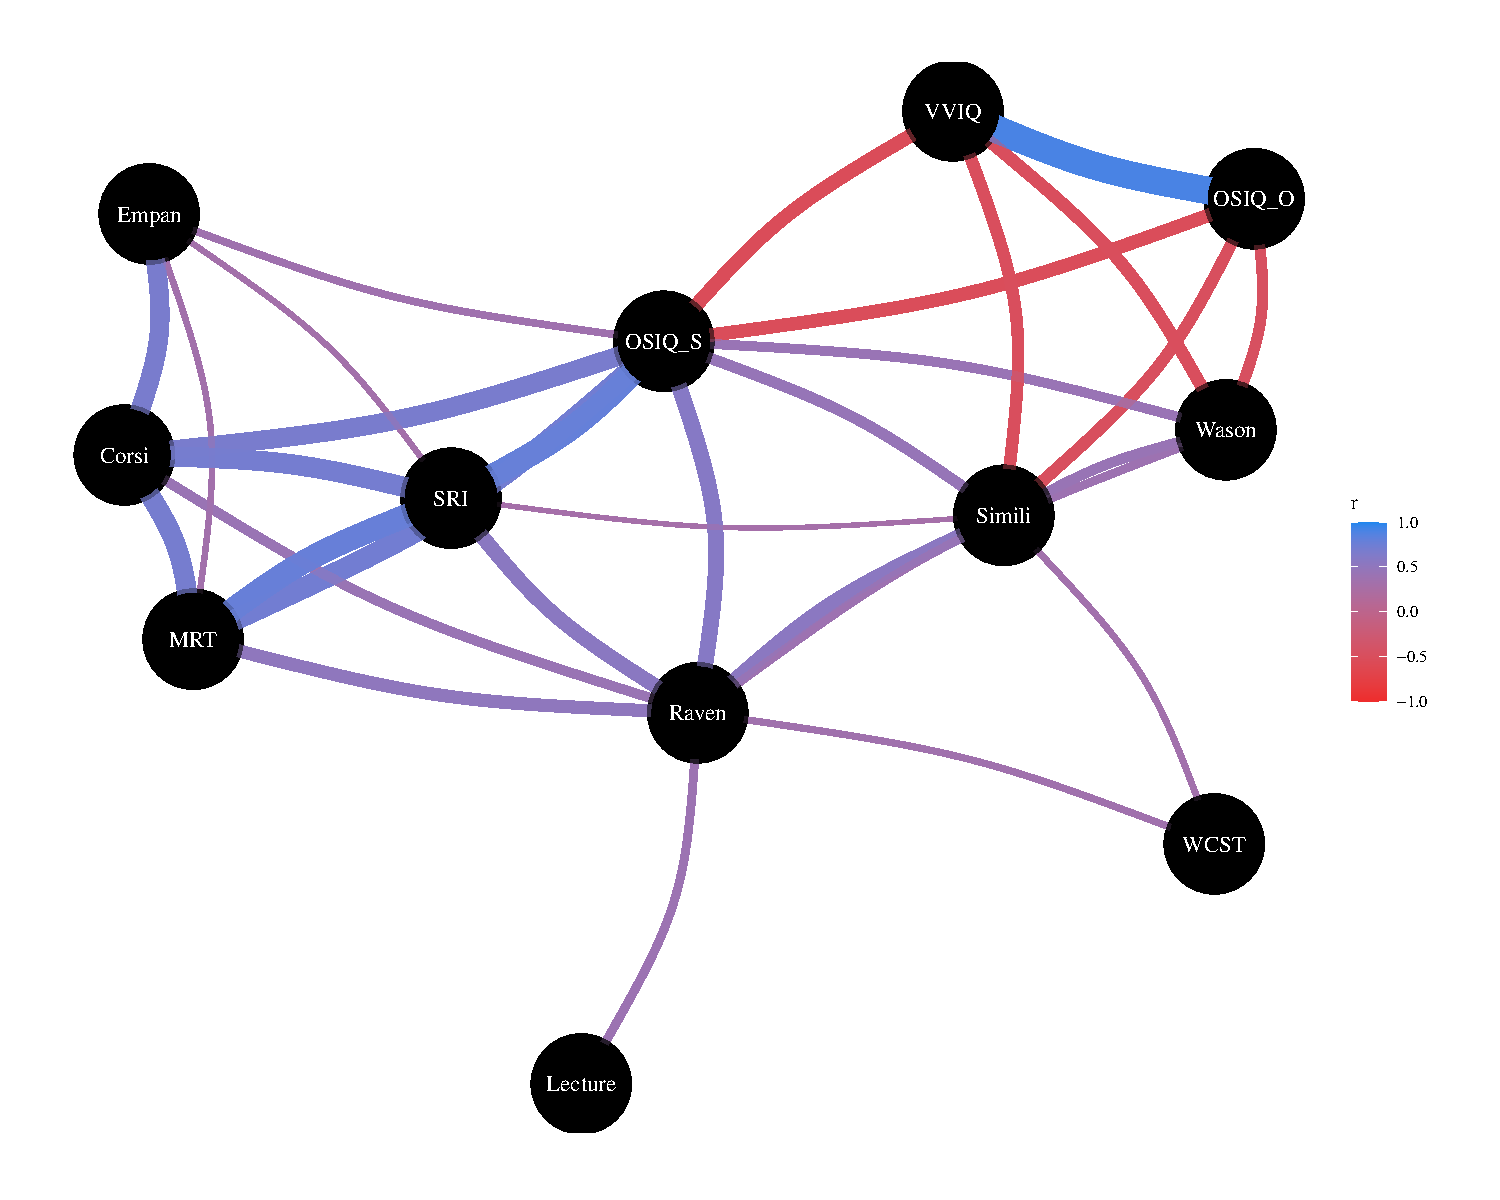
\includegraphics[width=\textwidth,height=0.5\textheight]{simu_0_aphantasia_files/figure-pdf/ggm_graph-1.pdf}

\caption{Représentation du GGM ajusté sur nos données. Chaque noeud représente une variable. Les liens bleus dénotent une corrélation positive, les rouges une corrélation négative, et leur épaisseur dépend de la force de cette corrélation. Le modèle illustre les choix de pondération réalisés à l'étape de simulation : on peut notamment voir des corrélations très prononcées entre le VVIQ et l'OSIQ-objet (r = 0.77, p<.001) qui évaluent tous deux l'imagerie objet, le Digit Span et les blocs de Corsi (r = 0.68, p<.001) qui évaluent entre autres la mémoire de travail, ou encore entre l'OSIQ-spatial et le SRI, qui sont respectivement l'auto-évaluation et la tâche les plus spécifiques de l'imagerie spatiale.}
\label{ggm_graph}
\end{figure}

Nous avons évalué que les données étaient adaptées à une analyse
factorielle multiple avec plusieurs indices. La mesure Kaiser, Meyer,
Olkin (KMO) de l'adéquation de l'échantillonnage suggère que les données
semblent appropriées à une analyse factorielle (KMO = 0,82), et le test
de sphéricité de Bartlett suggère qu'il y a une corrélation
significative suffisante dans les données pour une analyse factorielle
(Chisq(66) = 3194.04, p \textless{} .001). Ces deux indices ont été
calculés avec la fonction \texttt{check\_factorstructure} du package
\emph{parameters}.

Le choix de trois dimensions pour l'analyse était soutenu par cinq
(35,71\%) méthodes sur quatorze (dont CNG, coordonnées optimales,
analyse parallèle, critère de Kaiser, Scree (SE)).\footnote{Nous avons
  par ailleurs mené une analyse à quatre facteurs, dans la mesure où ce
  nombre était le deuxième le plus supporté par les indices de
  détermination : la quatrième dimension identifiée par cette analyse
  rassemble quasi-exclusivement les scores au Corsi et à l'Empan Verbal,
  soit les deux tâches de mémoire de travail. Voir la
  \autoref{loadings_graph_annex} en \nameref{annexes}. Les 4 facteurs
  latents ont représenté 67,82\% de la variance totale des données
  originales (MR1 = 25,86\%, MR2 = 21,57\%, MR3 = 12,91\%, MR4 =
  7,48\%).}. Nous avons donc conduit l'analyse factorielle multiple avec
la fonction \texttt{factor\_analysis} du package \emph{parameters} sur
R, réglée pour trois facteurs et une rotation ``clusters''. La
\autoref{loadings_tbl} présente les capacités explicatives de chaque
composante sur la variance de totale de l'échantillon. Les 3 facteurs
latents ont représenté 62,55\% de la variance totale des données
originales (MR1 = 26,91\%, MR2 = 21,53\%, MR3 = 14,11\%). La
distribution des poids de chaque variable selon les facteurs est
présentée en \autoref{loadings_graph}.

\begin{longtable}[]{@{}lrrr@{}}
\toprule()
Parameter & MR1 & MR2 & MR3 \\
\midrule()
\endfirsthead
\toprule()
Parameter & MR1 & MR2 & MR3 \\
\midrule()
\endhead
Eigenvalues & 4.545 & 2.000 & 0.961 \\
Variance & 0.269 & 0.215 & 0.141 \\
Variance\_Cumulative & 0.269 & 0.484 & 0.626 \\
Variance\_Proportion & 0.430 & 0.344 & 0.226 \\
\bottomrule()
\caption{Analyses des performances en termes de variance expliquée des
facteurs détérminés selon une rotation adaptée à une analyse de
clusters.\label{loadings_tbl}}\tabularnewline
\end{longtable}

\begin{figure}[h]

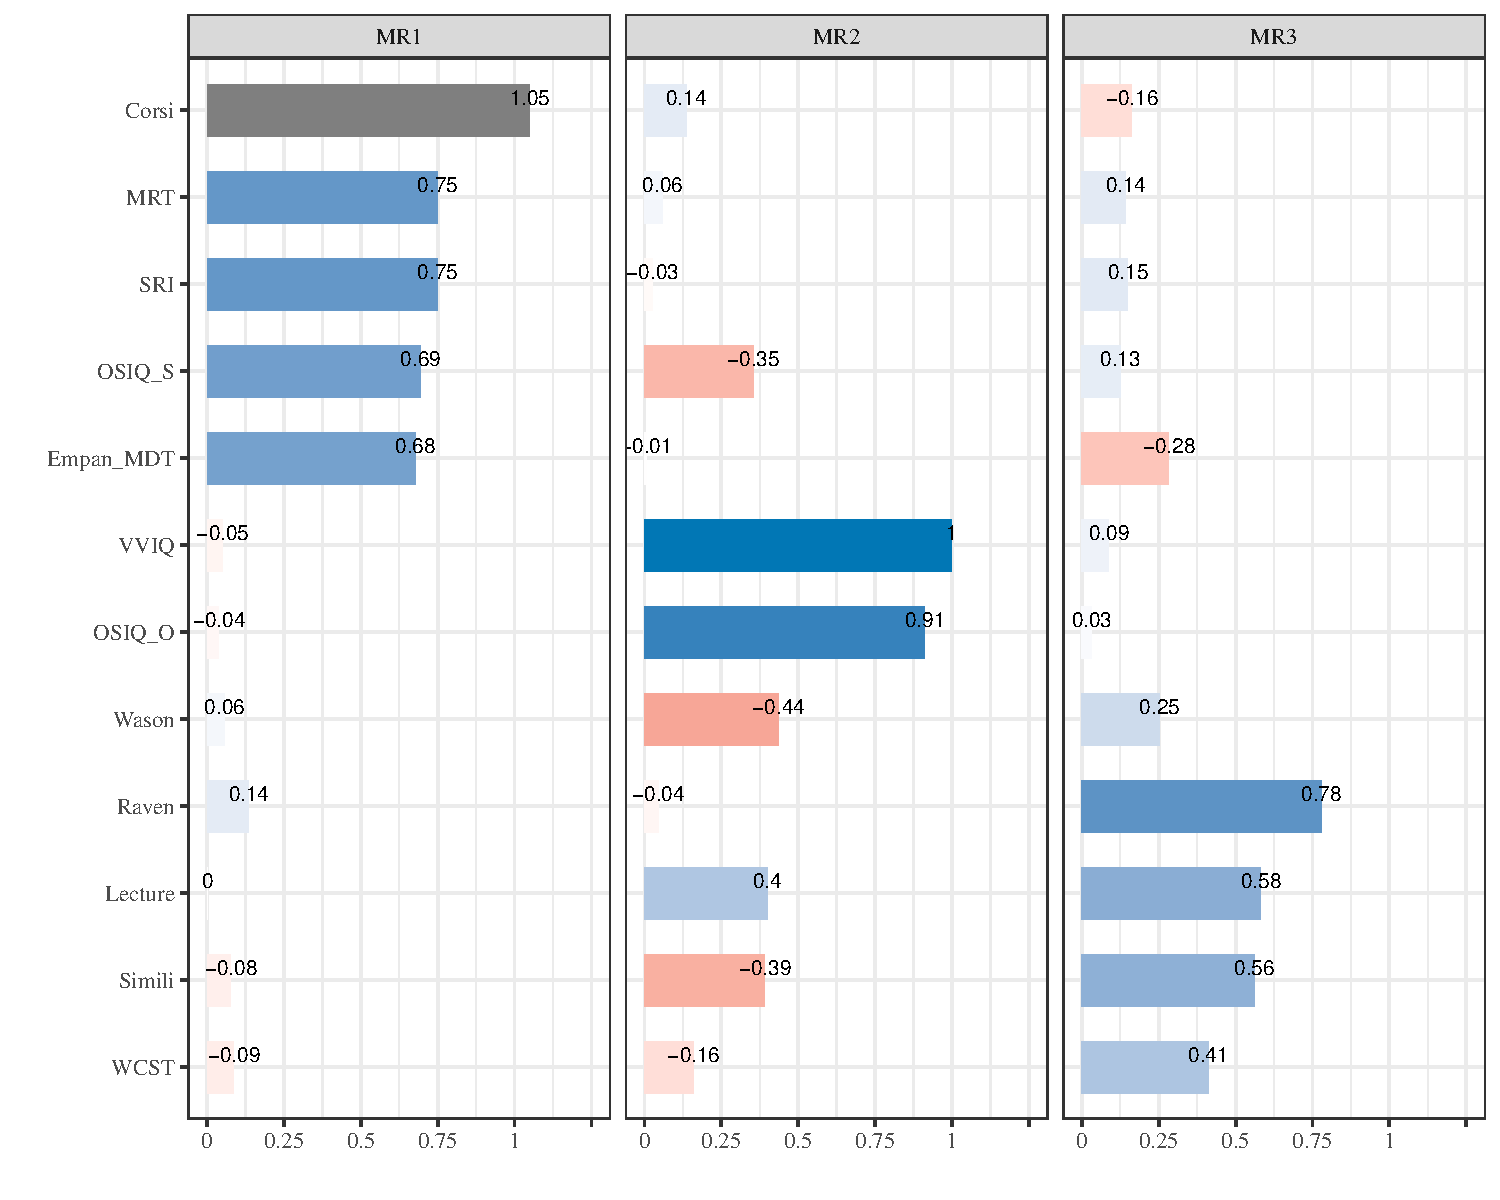
\includegraphics[width=\textwidth,height=0.5\textheight]{simu_0_aphantasia_files/figure-pdf/loadings_graph-1.pdf}

\caption{Poids de chaque variable dans l'Analyse Factorielle Multiple à trois facteurs.}
\label{loadings_graph}
\end{figure}

A partir de cette distribution et de l'analyse en graphes de nos
facteurs, nous avons catégorisé les trois composantes : la première, la
plus corrélée au SRI, au MRT, à l'OSIQ-Spatial et aux blocs de Corsi
(toutes des tâches ayant une composante spatiale) sera appelée
\textbf{Imagerie Spatiale}. La seconde, corrélée au VVIQ, à l'OSIQ-Objet
et au Wason, sera l'\textbf{Imagerie Objet}. La dernière, corrélée aux
Matrices de Raven, aux Similitudes, à la compréhension en lecture et au
WCST, sera le \textbf{Raisonnement}.

\hypertarget{analyse-en-clusters}{%
\subsubsection{\texorpdfstring{Analyse en
\emph{clusters}}{Analyse en clusters}}\label{analyse-en-clusters}}

Nous avons vérifié si l'ensemble de données était approprié pour le
clustering via la statistique H de Hopkins : H = 0.23. Si la valeur de
la statistique de Hopkins est proche de 0 (inférieure à 0,5), alors nous
pouvons rejeter l'hypothèse nulle et conclure que l'ensemble de données
est significativement clusterisable. Une valeur de H inférieure à 0,25
indique une tendance au clustering au niveau de confiance de 90\%
(\protect\hyperlink{ref-lawsonNewIndexClustering1990}{Lawson \& Jurs,
1990}).

Le nombre de clusters optimal a été calculé grâce à l'ensemble des
indices présents dans le package R NbClus
(\protect\hyperlink{ref-charradNbClustPackageDetermining2014}{Charrad et
al., 2014}). 38\% indices (11 sur 29) proposait un nombre optimal de
deux clusters pour notre échantillon, reflétant nos connaissances
\emph{a priori} et la construction de notre structure de facteurs sur la
base dichotomique aphantasiques/non-aphantasiques que nous connaissons.
Néanmoins, 27.5\% des indices (8 sur 29 - Elbow, Silhouette, Ch, CCC,
Cindex, DB, Duda, Pseudot2) soutenaient le choix de 4 clusters. A des
fins exploratoires, et pour mettre en évidence l'intérêt potentiel de
notre démarche analytique, nous avons décidé de mener nos analyses sur 4
clusters.

\begin{figure}[h]

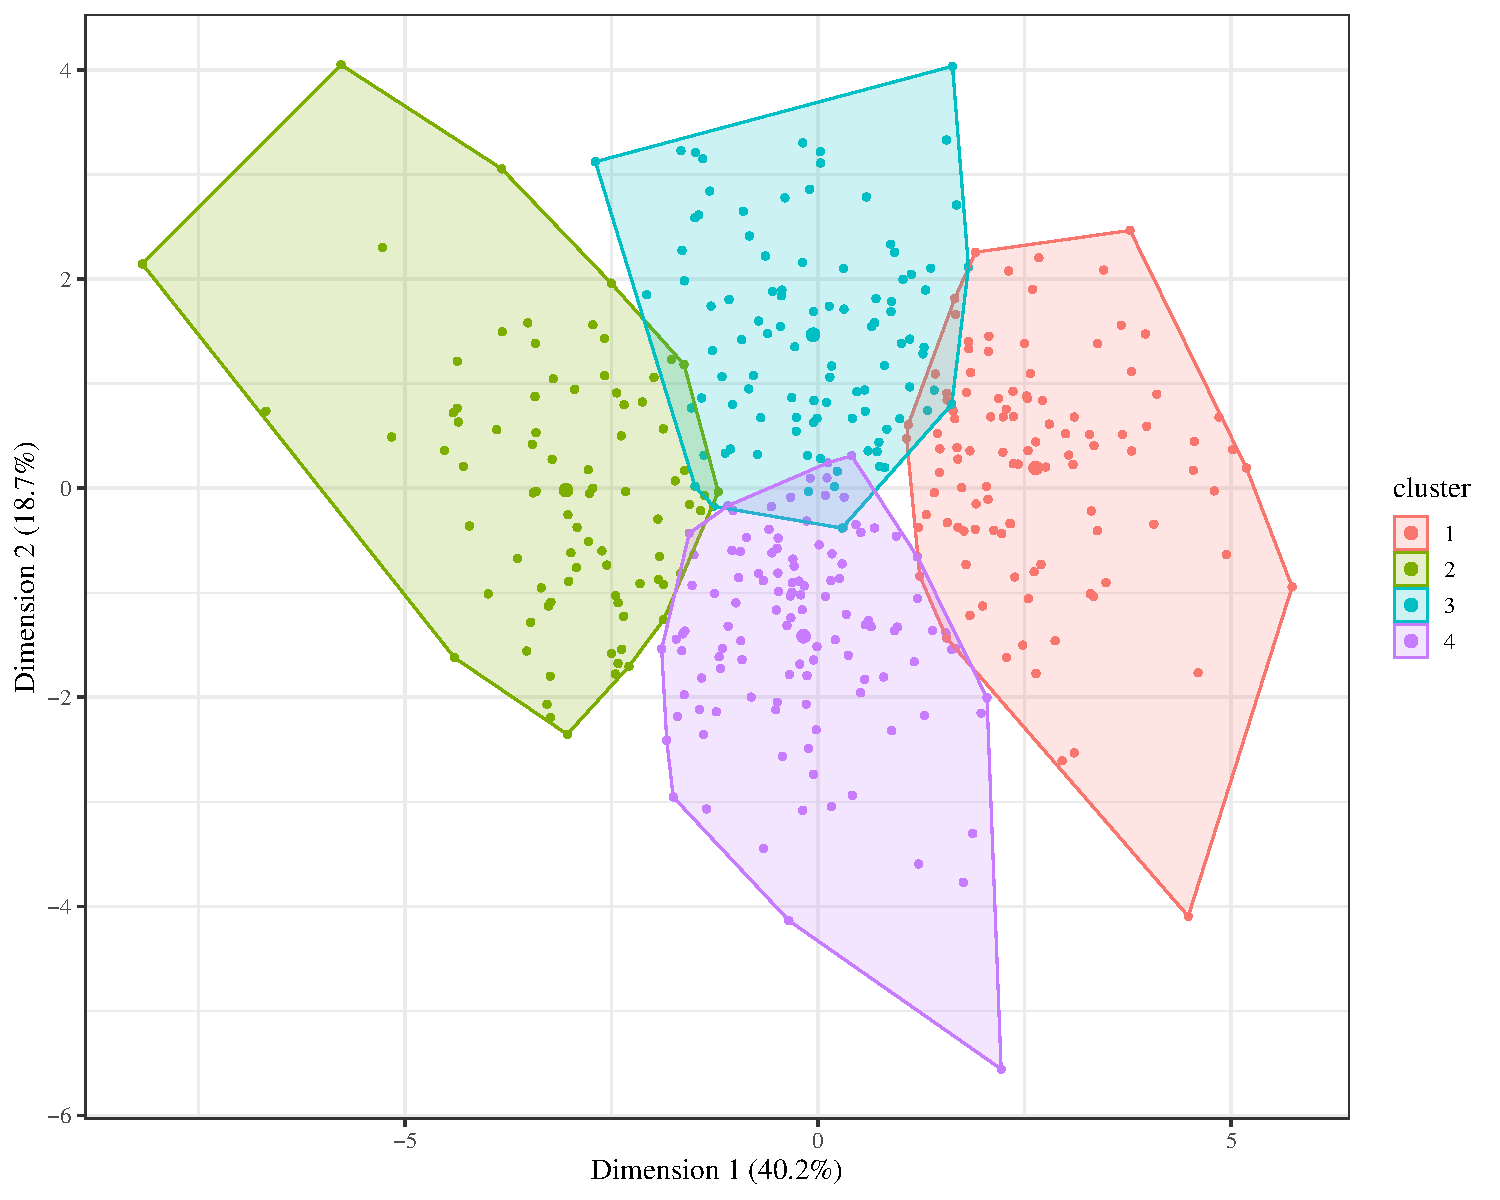
\includegraphics[width=\textwidth,height=0.5\textheight]{simu_0_aphantasia_files/figure-pdf/kmeans_plot-1.pdf}

\caption{Représentation des clusters reconnus par la méthode des 'k-means', selon les deux composantes principales de l'AFM.}
\label{kmeans_plot}
\end{figure}

Une implémentation de l'algorithme des \emph{k-means} a donc été
conduite avec 4 clusters sur l'ensemble de l'échantillon. Comme décrit
plus haut, suite au calcul de la matrice de dissimilarité, les
observations sont attribuées au cluster le plus probable en termes
d'assignation. L'algorithme entier est répété un grand nombre de fois (n
= 200 ici) avec des ``points de départ'' - l'endroit d'initialisation
des centres des clusters - différents. La partition choisie place chaque
participant dans le cluster où il était ``majoritairement'' sur toutes
les répétitions. Le résultat des k-means est représenté dans la
\autoref{kmeans_plot}, et les profils cognitifs associés sur les trois
capacités définies par l'AFM est en \autoref{radar}.

Par ailleurs, l'analyse de clusters montre que les quatre clusters
expliquent 60,70\% de la variance totale des données originales. Nous
avons alors mené une analyse comparative avec la solution à deux
clusters, qui n'expliqueraient ``que'' 37,26\% de la variance totale des
données, s'ajoutant à l'argumentaire de notre choix de quatre clusters.

\begin{figure}[h]

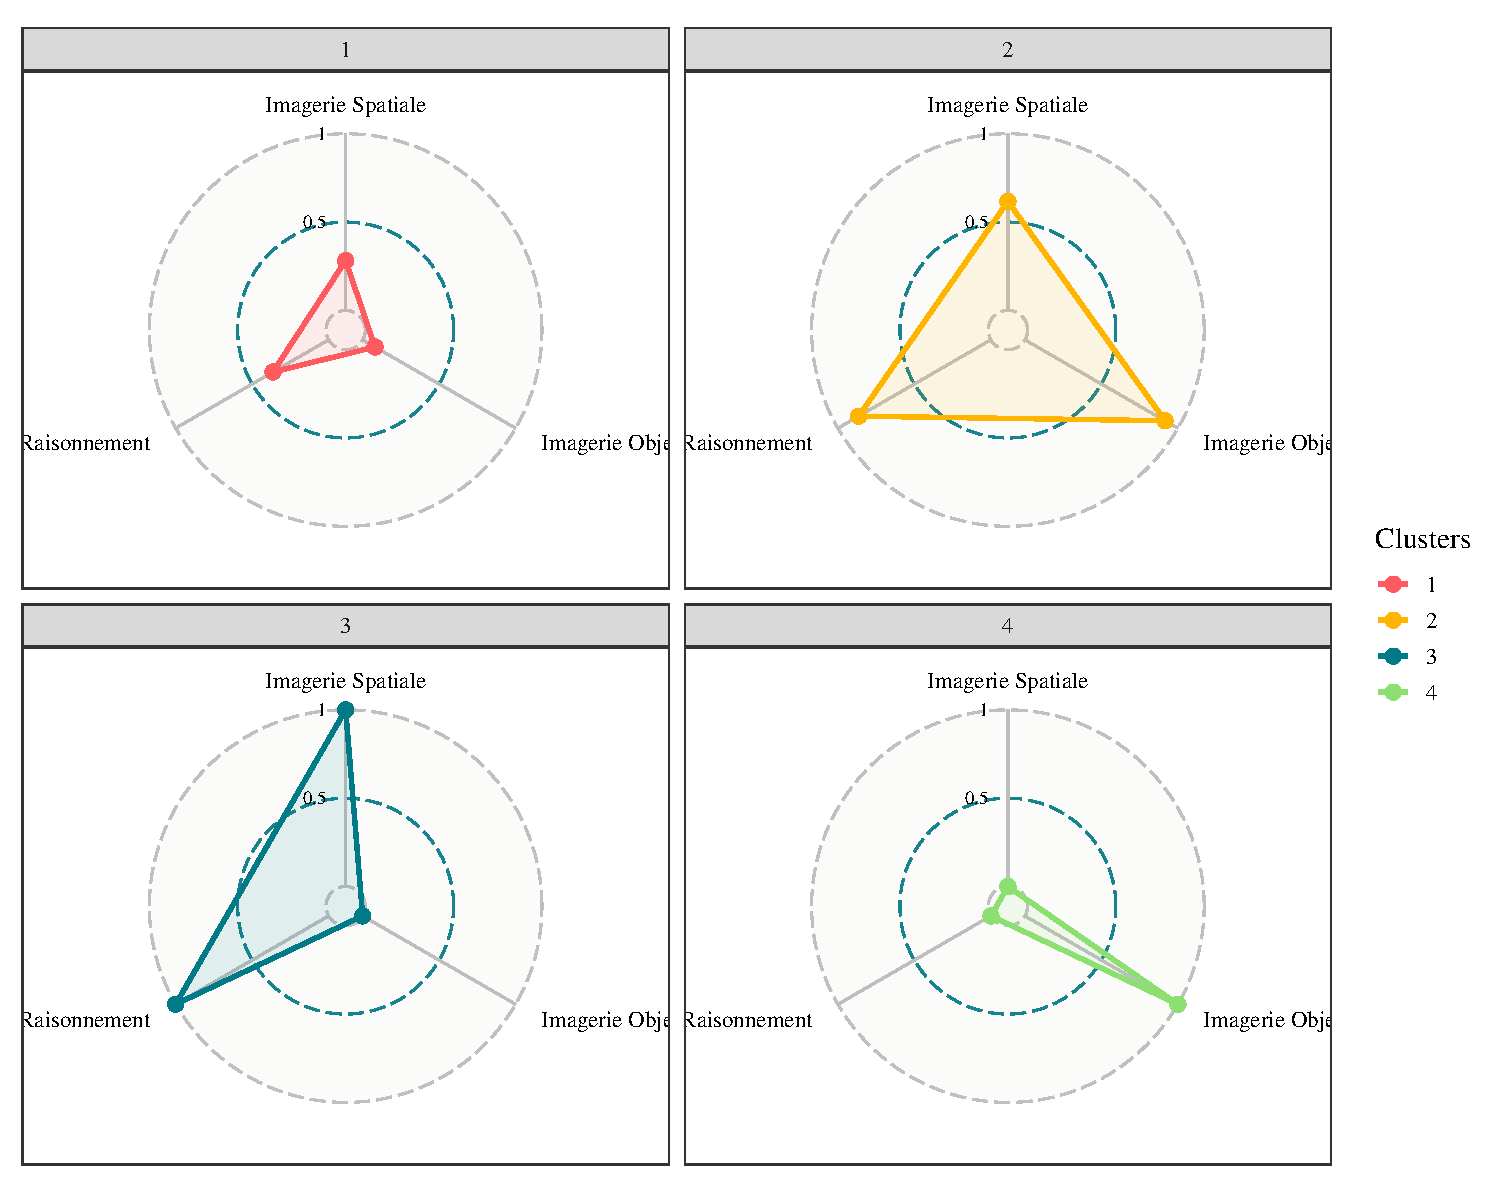
\includegraphics[width=1\textwidth,height=0.5\textheight]{simu_0_aphantasia_files/figure-pdf/radar-1.pdf}

\caption{Diagramme représentatant les profils cognitifs associés à chaque cluster, selon  trois dimensions principales : l'imagerie visuelle-objet, l'imagerie visuo-spatiale et le raisonnement.}
\label{radar}
\end{figure}

\hypertarget{composition-et-description-des-clusters}{%
\subsubsection{Composition et description des
clusters}\label{composition-et-description-des-clusters}}

Les profils ont ensuite été étudiés sur leur composition en fonction du
diagnostic initial et sur les compétences cognitives du profil et celles
sous-tendant ces performances grâce à des comparaisons de groupes.

La \autoref{repartition} présente la répartition dans les nouveaux
clusters des participants initialement identifiés comme aphantasiques ou
non par le VVIQ. Les clusters 3 et 4 sont représentatifs de l'importance
du critère de l'imagerie visuelle-objet : ils sont composés
respectivement de 100\% de contrôles et de 100\% d'aphantasiques. Les
clusters 1 et 2 sont néanmoins plus équilibrés.

Dans le but d'interpréter les clusters à partir des scores des
compétences les composant, une moyenne en dessous de 0 (moyenne
standardisée) est considérée comme déficitaire et une moyenne au-dessus
de 0 comme non-déficitaire. Les moyennes de chaque cluster aux variables
avec les tailles d'effectif sont présentés dans la
\autoref{repartition}.

\begin{longtable}[]{@{}
  >{\raggedright\arraybackslash}p{(\columnwidth - 10\tabcolsep) * \real{0.0930}}
  >{\raggedleft\arraybackslash}p{(\columnwidth - 10\tabcolsep) * \real{0.2093}}
  >{\raggedleft\arraybackslash}p{(\columnwidth - 10\tabcolsep) * \real{0.1744}}
  >{\raggedleft\arraybackslash}p{(\columnwidth - 10\tabcolsep) * \real{0.1512}}
  >{\raggedleft\arraybackslash}p{(\columnwidth - 10\tabcolsep) * \real{0.1628}}
  >{\raggedleft\arraybackslash}p{(\columnwidth - 10\tabcolsep) * \real{0.2093}}@{}}
\toprule()
\begin{minipage}[b]{\linewidth}\raggedright
Cluster
\end{minipage} & \begin{minipage}[b]{\linewidth}\raggedleft
Imagerie Spatiale
\end{minipage} & \begin{minipage}[b]{\linewidth}\raggedleft
Imagerie Objet
\end{minipage} & \begin{minipage}[b]{\linewidth}\raggedleft
Raisonnement
\end{minipage} & \begin{minipage}[b]{\linewidth}\raggedleft
Aphantasiques
\end{minipage} & \begin{minipage}[b]{\linewidth}\raggedleft
Non-Aphantasiques
\end{minipage} \\
\midrule()
\endfirsthead
\toprule()
\begin{minipage}[b]{\linewidth}\raggedright
Cluster
\end{minipage} & \begin{minipage}[b]{\linewidth}\raggedleft
Imagerie Spatiale
\end{minipage} & \begin{minipage}[b]{\linewidth}\raggedleft
Imagerie Objet
\end{minipage} & \begin{minipage}[b]{\linewidth}\raggedleft
Raisonnement
\end{minipage} & \begin{minipage}[b]{\linewidth}\raggedleft
Aphantasiques
\end{minipage} & \begin{minipage}[b]{\linewidth}\raggedleft
Non-Aphantasiques
\end{minipage} \\
\midrule()
\endhead
1 & -0.2435470 & -0.7742495 & -0.1801197 & 29 & 49 \\
2 & 0.4247462 & 0.7090962 & 0.6260035 & 42 & 73 \\
3 & 1.1891565 & -0.9185303 & 0.8451114 & 126 & 0 \\
4 & -0.8051109 & 0.8581758 & -0.7664169 & 0 & 81 \\
\bottomrule()
\caption{Moyennes évaluées à chaque compétence et répartion des
effectifs par cluster.\label{repartition}}\tabularnewline
\end{longtable}

Nous pourrons par la suite mener des analyses plus poussées par cluster
pour raffiner la description de chaque profil et son fonctionnement
(notamment tester des liens potentiels avec les statistiques
démographiques), mais celles-ci présenteraient peu d'intérêt dans le cas
présent, les données simulées ne représentant personne.

Dans l'objectif de mieux décrire les sous-groupes, nous réaliserons des
analyses de variance univariées. Nous avons ajusté des modèles linéaires
sur nos données pour prédire les nouveaux scores de \emph{Raisonnement},
d'\emph{Imagerie Objet} et d'\emph{Imagerie Spatiale} en fonction des
clusters, et ainsi mieux comparer et caractériser nos sous-groupes. Ces
modèles ont permis d'expliquer une part de variance importante et
statistiquement significative des scores en Raisonnement (\(r^2\) =
0.49, \emph{F}(3, 396) = 128.86, \emph{p} \textless{} .001, adj. \(r^2\)
ajusté = 0.49), en Imagerie Objet (\(r^2\) = 0.69, \emph{F}(3, 396) =
290.12, \emph{p}\textless{} .001, \(r^2\) ajusté = 0.68) et en Imagerie
Spatiale (\(r^2\) = 0.56, \emph{F}(3, 396) = 168.39, \emph{p}
\textless{} .001, \(r^2\) ajusté = 0.56).

A cette étape, les post-hoc des modèles avec un intercept à 0 nous
permettent de retrouver les valeurs de la \autoref{repartition}. Dans
l'analyse effective, nous réaliserions \emph{tendanciellement} (\emph{p}
= .06) des post-hocs deux-à-deux plus ciblés avec la correction que nous
choisirons : néanmoins dans ces analyses prévisionnelles, tout est
extrêmement significatif par construction et ces tests seraient
inutilement lourds. La \autoref{lollipop} présente les comparaisons des
différentes moyennes dans un histogramme de type \emph{Cleveland} (dit
\emph{lollipop chart}).

\begin{figure}[h]

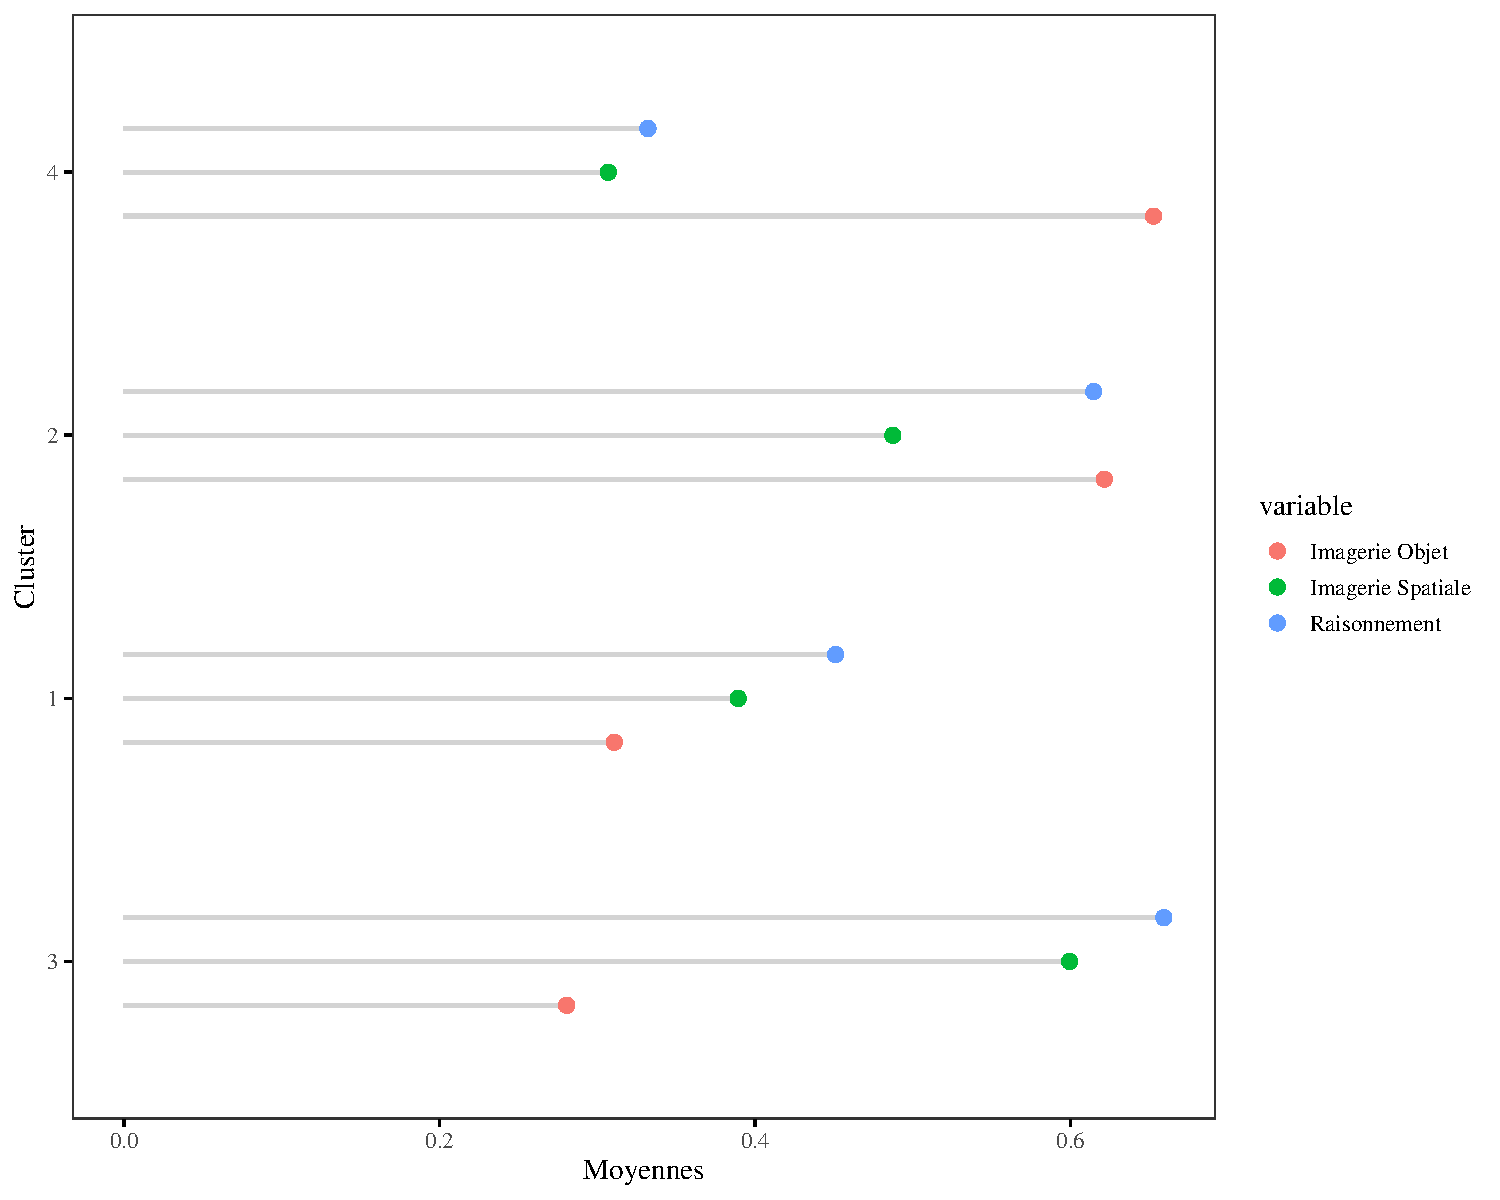
\includegraphics[width=\textwidth,height=0.5\textheight]{simu_0_aphantasia_files/figure-pdf/lollipop-1.pdf}

\caption{Représentation des moyennes de chaque cluster pour les trois capacités cognitives.}
\label{lollipop}
\end{figure}

\hypertarget{discussion}{%
\section{Discussion}\label{discussion}}

\hypertarget{une-analyse-exploratoire-de-limagerie-mentale.}{%
\subparagraph{Une analyse exploratoire de l'imagerie
mentale.}\label{une-analyse-exploratoire-de-limagerie-mentale.}}

L'analyse dimensionnelle \emph{data driven} peut mettre en évidence des
liens entre des capacités cognitives à partir des données : elle
pourrait permettre d'élucider les connections des différentes formes de
l'imagerie entre elles et avec les compétences abstraites. Une analyse
factorielle puis basée sur la théorie des graphes permettrait de lier
les compétences individuelles en des réseaux fonctionnels cohérents dont
la proximité ou la distance serait mise en évidence sans interférence
des nos hypothèses.\\
Dans cette simulation (dont la base est bien sûr teintée par toutes les
connaissances et hypothèses \emph{a priori}), l'Analyse Factorielle
Multiple a permis de mettre en évidence trois composantes cognitives
reflétées par nos facteurs: l'imagerie visuelle-objet, l'imagerie
visuospatiale et le raisonnement. La pertinence analytique de la méthode
est reflétée par la différence entre notre méthodologie de simulation et
le résultat de l'AFM : nous avions initialement simulé douze variables
et les avions liées linéairement à cinq facteurs latents, pondération
qui était dépendante de nos présuppositions sur les facteurs en
question. L'AFM en a extrait trois très pertinents, mais avait aussi
identifié - dans un quatrième facteur moins impactant - la \emph{mémoire
de travail}. L'autre facteur que nous avions construit, la
\emph{flexibilité mentale}, a été évacué par l'analyse de facteurs car
indiscernable des autres : nos variables étaient toutes plus corrélées à
d'autres facteurs qu'à la flexibilité elle-même. L'analyse successive en
graphes par un \emph{Gaussian Graphical Model} nous a permis d'observer
les distances entre ces réseaux et leur liens réciproques. Sur la base
d'une matrice corrélation entre les variables, elle a créé une analyse
géométrique du plan de facteurs et une représentation de celui-ci. Cette
représentation a montré sa capacité à révéler des liens entre variables
mais aussi entre \emph{réseaux}. Dans notre simulation nous avions par
exemple créé intentionnellement\footnote{Ces phénomènes n'existaient que
  de façon sous-jacente à nos coefficients du modèle factoriel,
  i.e.~dans notre modèle d'\emph{effets}.} deux phénomènes : une
corrélation négative entre l'imagerie visuelle-objet d'un côté et
l'imagerie spatiale et le raisonnement de l'autre, ainsi qu'une
corrélation positive entre l'imagerie spatiale et le raisonnement. Ces
deux phénomènes sont très bien retranscrits par le GGM, illustrant sa
pertinence dans de tels modèles de données.

\hypertarget{vers-la-construction-de-profils-cognitifs-des-aphantasies}{%
\paragraph{Vers la construction de profils cognitifs des
aphantasies}\label{vers-la-construction-de-profils-cognitifs-des-aphantasies}}

Nos données - illustrant notre recrutement réel potentiel - étaient ici
construites sur la base de deux sets de moyennes représentant deux
groupes \emph{supposés}, divisés selon un axe d'une seule dimension : le
déficit (ou non) d'imagerie visuelle (objet). Cette étude a permis de
démontrer la pertinence de l'intervention d'un algorithme de partition
non-supervisée (\emph{k-means}) pour redéfinir les groupes - si
nécessaire - sur plusieurs dimensions en partant des données elles-mêmes
et en s'affranchissant alors de nos connaissances préalables. Nous avons
ici illustré une situation potentielle ou cette partition résulte en une
recommandation de quatre groupes au lieu de deux. Du fait de la
construction manuelle des données, ces groupes ont des caractéristiques
exagérées. Néanmoins nous pouvons dégager le sens de la partition
réalisée par l'algorithme (voir \autoref{radar}). Il existe deux groupes
performants en raisonnement : un groupe performant à toutes les
compétences (le cluster 2), composé majoritairement de non-aphantasiques
- ceux-ci représentent les contrôles moyens et les aphantasiques
``indiscernables''. Il existe ensuite un groupe - le cluster 3 - très
faible en imagerie objet mais encore davantage performant en
raisonnement et imagerie spatiale, composé uniquement d'aphantasiques :
il reflète les aphantasiques de ``haut niveau'' et illustre l'équilibre
potentiellement avantageux des stratégies alternatives des
aphantasiques\footnote{Ce serait ici notre groupe
  d'``\emph{aphantasiques scientifiques}''.}. Le cluster 1 est mixte
mais composé majoritairement de non-aphantasiques, et représente la
moyenne basse des ``compétences équilibrées'' et des aphantasiques
``indiscernables''. Enfin le cluster 4, composé uniquement de
non-aphantasiques, présente des moyennes très basses sauf en
imagerie-objet, où il présente la moyenne la plus élevée : ce serait ici
nos ``hyperphantasiques''.

Le plan d'analyse et les simulations présentées ici ont permis de mettre
en évidence l'intérêt dans un premier temps d'une étude dimensionnelle
et exploratoire \emph{data-driven} des compétences de l'imagerie et de
l'abstraction, puis d'une analyse des données des participants
partitionnées de façon non-supervisée. Nous avons ainsi établi avec ce
dossier qu'un tel plan d'étude et d'analyse semble prometteur et fécond
: ce plan sera potentiellement mis en application dès le deuxième
trimestre 2023 dans l'étude réelle.

\newpage

\hypertarget{ruxe9fuxe9rences}{%
\section*{Références}\label{ruxe9fuxe9rences}}
\addcontentsline{toc}{section}{Références}

\hypertarget{refs}{}
\begin{CSLReferences}{1}{0}
\leavevmode\vadjust pre{\hypertarget{ref-R-quarto}{}}%
Allaire, J. (2022). \emph{Quarto: {R} Interface to Quarto Markdown
Publishing System} {[}Manual{]}.
\url{https://github.com/quarto-dev/quarto-r}

\leavevmode\vadjust pre{\hypertarget{ref-R-rmarkdown}{}}%
Allaire, J., Xie, Y., McPherson, J., Luraschi, J., Ushey, K., Atkins,
A., Wickham, H., Cheng, J., Chang, W., \& Iannone, R. (2023).
\emph{Rmarkdown: {Dynamic} Documents for {R}} {[}Manual{]}.
\url{https://CRAN.R-project.org/package=rmarkdown}

\leavevmode\vadjust pre{\hypertarget{ref-bainbridgeQuantifyingAphantasiaDrawing2021}{}}%
Bainbridge, W. A., Pounder, Z., Eardley, A. F., \& Baker, C. I. (2021).
Quantifying Aphantasia through Drawing: {Those} without Visual Imagery
Show Deficits in Object but Not Spatial Memory. \emph{Cortex},
\emph{135}, 159‑172. \url{https://doi.org/10.1016/j.cortex.2020.11.014}

\leavevmode\vadjust pre{\hypertarget{ref-bartolomeoAssessingCausalRole2020}{}}%
Bartolomeo, P., Hajhajate, D., Liu, J., \& Spagna, A. (2020). Assessing
the Causal Role of Early Visual Areas in Visual Mental Imagery.
\emph{Nature Reviews Neuroscience}, \emph{21}(9, 9), 517‑517.
\url{https://doi.org/10.1038/s41583-020-0348-5}

\leavevmode\vadjust pre{\hypertarget{ref-R-effectsize}{}}%
Ben-Shachar, M. S., Makowski, D., Lüdecke, D., Patil, I., Wiernik, B.
M., \& Th'eriault, R. (2023). \emph{Effectsize: {Indices} of Effect
Size} {[}Manual{]}. \url{https://easystats.github.io/effectsize/}

\leavevmode\vadjust pre{\hypertarget{ref-bhushanUsingGaussianGraphical2019}{}}%
Bhushan, N., Mohnert, F., Sloot, D., Jans, L., Albers, C., \& Steg, L.
(2019). Using a {Gaussian Graphical Model} to {Explore Relationships
Between Items} and {Variables} in {Environmental Psychology Research}.
\emph{Frontiers in Psychology}, \emph{10}.
\url{https://www.frontiersin.org/articles/10.3389/fpsyg.2019.01050}

\leavevmode\vadjust pre{\hypertarget{ref-bilkerDevelopmentAbbreviatedNineItem2012}{}}%
Bilker, W. B., Hansen, J. A., Brensinger, C. M., Richard, J., Gur, R.
E., \& Gur, R. C. (2012). Development of {Abbreviated Nine-Item Forms}
of the {Raven}'s {Standard Progressive Matrices Test}.
\emph{Assessment}, \emph{19}(3), 354‑369.
\url{https://doi.org/10.1177/1073191112446655}

\leavevmode\vadjust pre{\hypertarget{ref-R-ggradar}{}}%
Bion, R. (2023). \emph{Ggradar: {Create} Radar Charts Using Ggplot2}
{[}Manual{]}.

\leavevmode\vadjust pre{\hypertarget{ref-blajenkovaObjectSpatialImagery2006}{}}%
Blajenkova, O., Kozhevnikov, M., \& Motes, M. A. (2006a). Object and
Spatial Imagery: Distinctions between Members of Different Professions.
\emph{Cognitive Processing}, \emph{7}(1), 20‑21.
\url{https://doi.org/10.1007/s10339-006-0047-9}

\leavevmode\vadjust pre{\hypertarget{ref-blajenkovaObjectspatialImageryNew2006}{}}%
Blajenkova, O., Kozhevnikov, M., \& Motes, M. A. (2006b). Object-Spatial
Imagery: A New Self-Report Imagery Questionnaire. \emph{Applied
Cognitive Psychology}, \emph{20}(2), 239‑263.
\url{https://doi.org/10.1002/acp.1182}

\leavevmode\vadjust pre{\hypertarget{ref-blazhenkovaVisualobjectAbilityNew2010}{}}%
Blazhenkova, O., \& Kozhevnikov, M. (2010). Visual-Object Ability: {A}
New Dimension of Non-Verbal Intelligence. \emph{Cognition},
\emph{117}(3), 276‑301.
\url{https://doi.org/10.1016/j.cognition.2010.08.021}

\leavevmode\vadjust pre{\hypertarget{ref-blazhenkovaNewObjectspatialverbalCognitive2009}{}}%
Blazhenkova, O., \& Kozhevnikov, M. (2009). The New
Object-Spatial-Verbal Cognitive Style Model: {Theory} and Measurement.
\emph{Applied Cognitive Psychology}, \emph{23}(5), 638‑663.
\url{https://doi.org/10.1002/acp.1473}

\leavevmode\vadjust pre{\hypertarget{ref-blomkvistAphantasiaSearchTheory2022}{}}%
Blomkvist, A. (2022). Aphantasia: {In} Search of a Theory. \emph{Mind \&
Language}, \emph{n/a}(n/a). \url{https://doi.org/10.1111/mila.12432}

\leavevmode\vadjust pre{\hypertarget{ref-brewerScientistsAreNot2006}{}}%
Brewer, W. F., \& Schommer-Aikins, M. (2006). Scientists {Are Not
Deficient} in {Mental Imagery}: {Galton Revised}. \emph{Review of
General Psychology}, \emph{10}(2), 130‑146.
\url{https://doi.org/10.1037/1089-2680.10.2.130}

\leavevmode\vadjust pre{\hypertarget{ref-cavedon-taylorPredictiveProcessingPerception2021}{}}%
Cavedon-Taylor, D. (2021). \emph{Predictive {Processing} and
{Perception}: {What} Does {Imagining} Have to Do with It?} 15.

\leavevmode\vadjust pre{\hypertarget{ref-charradNbClustPackageDetermining2014}{}}%
Charrad, M., Ghazzali, N., Boiteau, V., \& Niknafs, A. (2014).
{NbClust}: An {R} Package for Determining the Relevant Number of
Clusters in a Data Set. \emph{Journal of statistical software},
\emph{61}, 1‑36.

\leavevmode\vadjust pre{\hypertarget{ref-colemanSpatialPerceptionSkills1998}{}}%
Coleman, S. L., \& Gotch, A. J. (1998). Spatial {Perception Skills} of
{Chemistry Students}. \emph{Journal of Chemical Education},
\emph{75}(2), 206. \url{https://doi.org/10.1021/ed075p206}

\leavevmode\vadjust pre{\hypertarget{ref-crowderDifferencesSpatialVisualization2018}{}}%
Crowder, A. (2018). \emph{Differences in {Spatial Visualization Ability}
and {Vividness} of {Spatial Imagery Between People With} and {Without
Aphantasia}}.

\leavevmode\vadjust pre{\hypertarget{ref-danceLessSensoryOverwhelm2022}{}}%
Dance, C. (2022, janvier 26). \emph{Less {Sensory Overwhelm In
Aphantasia}: {A Potential Advantage}?}
\url{https://aphantasia.com/sensory-overwhelm/}

\leavevmode\vadjust pre{\hypertarget{ref-dancePrevalenceAphantasiaImagery2022}{}}%
Dance, C. J., Ipser, A., \& Simner, J. (2022). The Prevalence of
Aphantasia (Imagery Weakness) in the General Population.
\emph{Consciousness and Cognition}, \emph{97}, 103243.
\url{https://doi.org/10.1016/j.concog.2021.103243}

\leavevmode\vadjust pre{\hypertarget{ref-danceWhatLinkMental2021}{}}%
Dance, C. J., Ward, J., \& Simner, J. (2021). What Is the {Link Between
Mental Imagery} and {Sensory Sensitivity}? {Insights} from {Aphantasia}.
\emph{Perception}, \emph{50}(9), 757‑782.
\url{https://doi.org/10.1177/03010066211042186}

\leavevmode\vadjust pre{\hypertarget{ref-dawesInnerVisionsMind2022}{}}%
Dawes, A. (2022). \emph{Inner Visions of the Mind's Eye: {The} Role of
Visual Imagery in Remembering the Past and Imagining the Future}
{[}{UNSW Sydney}{]}. \url{https://doi.org/10.26190/UNSWORKS/24158}

\leavevmode\vadjust pre{\hypertarget{ref-dawesCognitiveProfileMultisensory2020}{}}%
Dawes, A. J., Keogh, R., Andrillon, T., \& Pearson, J. (2020). A
Cognitive Profile of Multi-Sensory Imagery, Memory and Dreaming in
Aphantasia. \emph{Scientific Reports}, \emph{10}(1, 1), 10022.
\url{https://doi.org/10.1038/s41598-020-65705-7}

\leavevmode\vadjust pre{\hypertarget{ref-R-pandoc}{}}%
Dervieux, C. (2022). \emph{Pandoc: {Manage} and Run Universal Converter
Pandoc from {R}} {[}Manual{]}.
\url{https://CRAN.R-project.org/package=pandoc}

\leavevmode\vadjust pre{\hypertarget{ref-farahCaseStudyMental1988}{}}%
Farah, M. J., Levine, D. N., \& Calvanio, R. (1988). A Case Study of
Mental Imagery Deficit. \emph{Brain and Cognition}, \emph{8}(2),
147‑164. \url{https://doi.org/10.1016/0278-2626(88)90046-2}

\leavevmode\vadjust pre{\hypertarget{ref-fawConflictingIntuitionsMay2009}{}}%
Faw, B. (2009). \emph{Conflicting {Intuitions May Be Based On Differing
Abilities}}. 25.

\leavevmode\vadjust pre{\hypertarget{ref-fox-muratonWorldImaginationConsequences2021}{}}%
Fox-Muraton, M. (2021). A World without Imagination? {Consequences} of
Aphantasia for an Existential Account of Self. \emph{History of European
Ideas}, \emph{47}(3), 414‑428.
\url{https://doi.org/10.1080/01916599.2020.1799553}

\leavevmode\vadjust pre{\hypertarget{ref-galtonSTATISTICSMENTALIMAGERY1880}{}}%
Galton, F. (1880). I.---{STATISTICS OF MENTAL IMAGERY}. \emph{Mind},
\emph{os-V}(19), 301‑318. \url{https://doi.org/10.1093/mind/os-V.19.301}

\leavevmode\vadjust pre{\hypertarget{ref-ganczarekRememberThingsCan2020}{}}%
Ganczarek, J., Żurawska-Żyła, R., \& Rolek, A. (2020). \emph{{«~I
remember things, but I can't picture them.~»} What can a case of
aphantasia tell us about imagery and memory?} \emph{20}(2), 134‑141.
\url{https://doi.org/10.15557/PiPK.2020.0018}

\leavevmode\vadjust pre{\hypertarget{ref-gibeauCorsiBlocksTask2021}{}}%
Gibeau, R.-M. (2021). The {Corsi Blocks Task}: {Variations} and Coding
with {jsPsych}. \emph{The Quantitative Methods for Psychology},
\emph{17}(3), 299‑311. \url{https://doi.org/10.20982/tqmp.17.3.p299}

\leavevmode\vadjust pre{\hypertarget{ref-greenbergRoleVisualImagery2014}{}}%
Greenberg, D. L., \& Knowlton, B. J. (2014). The Role of Visual Imagery
in Autobiographical Memory. \emph{Memory \& Cognition}, \emph{42}(6),
922‑934. \url{https://doi.org/10.3758/s13421-014-0402-5}

\leavevmode\vadjust pre{\hypertarget{ref-groegerMeasuringMemorySpan1999}{}}%
Groeger, J. A., Field, D., \& Hammond, S. M. (1999). Measuring Memory
Span. \emph{International Journal of Psychology}, \emph{34}(5-6),
359‑363. \url{https://doi.org/10.1080/002075999399693}

\leavevmode\vadjust pre{\hypertarget{ref-heatonWCST64ComputerVersion2000}{}}%
Heaton, R. K., \& Par, S. (2000). {WCST-64}: Computer Version 2.
\emph{PAR Psychological Assessment Resources, Lutz, FL}.

\leavevmode\vadjust pre{\hypertarget{ref-hegartyIndividualDifferencesSpatial2005}{}}%
Hegarty, M., \& Waller, D. A. (2005). Individual {Differences} in
{Spatial Abilities}. In \emph{The {Cambridge Handbook} of {Visuospatial
Thinking}} (p. 121‑169). {Cambridge University Press}.
\url{https://doi.org/10.1017/CBO9780511610448.005}

\leavevmode\vadjust pre{\hypertarget{ref-R-purrr}{}}%
Henry, L., \& Wickham, H. (2022). \emph{Purrr: {Functional} Programming
Tools} {[}Manual{]}. \url{https://CRAN.R-project.org/package=purrr}

\leavevmode\vadjust pre{\hypertarget{ref-junichiPreliminarySinglecaseStudy2020}{}}%
JUNICHI, T., \& JIRO, G. (2020). A Preliminary Single-Case Study of
Aphantasia in {Japan}. \emph{Tohoku Psychologica Folia}, \emph{79},
26‑32.

\leavevmode\vadjust pre{\hypertarget{ref-R-ggpubr}{}}%
Kassambara, A. (2022). \emph{Ggpubr: Ggplot2 Based Publication Ready
Plots} {[}Manual{]}. \url{https://rpkgs.datanovia.com/ggpubr/}

\leavevmode\vadjust pre{\hypertarget{ref-R-factoextra}{}}%
Kassambara, A., \& Mundt, F. (2020). \emph{Factoextra: {Extract} and
Visualize the Results of Multivariate Data Analyses} {[}Manual{]}.
\url{http://www.sthda.com/english/rpkgs/factoextra}

\leavevmode\vadjust pre{\hypertarget{ref-keehnerSpatialAbilityExperience2004}{}}%
Keehner, M. M., Tendick, F., Meng, M. V., Anwar, H. P., Hegarty, M.,
Stoller, M. L., \& Duh, Q.-Y. (2004). Spatial Ability, Experience, and
Skill in Laparoscopic Surgery. \emph{The American Journal of Surgery},
\emph{188}(1), 71‑75.
\url{https://doi.org/10.1016/j.amjsurg.2003.12.059}

\leavevmode\vadjust pre{\hypertarget{ref-kendleAphantasiaExperiencesPerceptions2017}{}}%
Kendle, A. (2017). \emph{Aphantasia: {Experiences}, Perceptions, and
Insights}. {Dark River}.

\leavevmode\vadjust pre{\hypertarget{ref-keoghBlindMindNo2018}{}}%
Keogh, R., \& Pearson, J. (2018). The Blind Mind: {No} Sensory Visual
Imagery in Aphantasia. \emph{Cortex}, \emph{105}, 53‑60.
\url{https://doi.org/10.1016/j.cortex.2017.10.012}

\leavevmode\vadjust pre{\hypertarget{ref-keoghAttentionDrivenPhantom2020}{}}%
Keogh, R., \& Pearson, J. (2020). Attention Driven Phantom Vision:
Measuring the Sensory Strength of Attentional Templates and Their
Relation to Visual Mental Imagery and Aphantasia. \emph{Philosophical
Transactions of the Royal Society B: Biological Sciences},
\emph{376}(1817), 20190688. \url{https://doi.org/10.1098/rstb.2019.0688}

\leavevmode\vadjust pre{\hypertarget{ref-keoghVisualWorkingMemory2021}{}}%
Keogh, R., Wicken, M., \& Pearson, J. (2021). Visual Working Memory in
Aphantasia: {Retained} Accuracy and Capacity with a Different Strategy.
\emph{Cortex}, \emph{143}, 237‑253.
\url{https://doi.org/10.1016/j.cortex.2021.07.012}

\leavevmode\vadjust pre{\hypertarget{ref-knauffVisualImageryCan2002}{}}%
Knauff, M., \& Johnson-Laird, P. N. (2002). Visual Imagery Can Impede
Reasoning. \emph{Memory \& Cognition}, \emph{30}(3), 363‑371.
\url{https://doi.org/10.3758/BF03194937}

\leavevmode\vadjust pre{\hypertarget{ref-knightMemoryImageryNo2022}{}}%
Knight, K. F., Milton, F. N., Milton, F. N., Zeman, A., \& Zeman, A.
(2022). \emph{Memory without {Imagery}: {No Evidence} of {Visual Working
Memory Impairment} in {People} with {Aphantasia}}. 8.

\leavevmode\vadjust pre{\hypertarget{ref-kosslynCognitiveNeuroscienceMental1995}{}}%
Kosslyn, S. M., Behrmann, M., \& Jeannerod, M. (1995). The Cognitive
Neuroscience of Mental Imagery. \emph{Neuropsychologia}, \emph{33}(11),
1335‑1344. \url{https://doi.org/10.1016/0028-3932(95)00067-D}

\leavevmode\vadjust pre{\hypertarget{ref-kotheTrackdownCollaborativeWriting2021}{}}%
Kothe, E., Callegher, C. Z., Gambarota, F., Linkersdörfer, J., \& Ling,
M. (2021). \emph{Trackdown: {Collaborative Writing} and {Editing} of {R
Markdown} (or {Sweave}) {Documents} in {Google Drive}}. {Zenodo}.
\url{https://doi.org/10.5281/zenodo.5167320}

\leavevmode\vadjust pre{\hypertarget{ref-kozhevnikovTradeoffObjectSpatial2010}{}}%
Kozhevnikov, M., Blazhenkova, O., \& Becker, M. (2010). Trade-off in
Object versus Spatial Visualization Abilities: {Restriction} in the
Development of Visual-Processing Resources. \emph{Psychonomic Bulletin
\& Review}, \emph{17}(1), 29‑35.
\url{https://doi.org/10.3758/PBR.17.1.29}

\leavevmode\vadjust pre{\hypertarget{ref-kozhevnikovSpatialObjectVisualizers2005}{}}%
Kozhevnikov, M., Kosslyn, S., \& Shephard, J. (2005). Spatial versus
Object Visualizers: {A} New Characterization of Visual Cognitive Style.
\emph{Memory \& Cognition}, \emph{33}(4), 710‑726.
\url{https://doi.org/10.3758/BF03195337}

\leavevmode\vadjust pre{\hypertarget{ref-kozhevnikovCreativityVisualizationAbilities2013}{}}%
Kozhevnikov, M., Kozhevnikov, M., Yu, C. J., \& Blazhenkova, O. (2013).
Creativity, Visualization Abilities, and Visual Cognitive Style.
\emph{British Journal of Educational Psychology}, \emph{83}(2), 196‑209.
\url{https://doi.org/10.1111/bjep.12013}

\leavevmode\vadjust pre{\hypertarget{ref-kozhevnikovSpatialVisualizationPhysics2007}{}}%
Kozhevnikov, M., Motes, M. A., \& Hegarty, M. (2007). Spatial
{Visualization} in {Physics Problem Solving}. \emph{Cognitive Science},
\emph{31}(4), 549‑579. \url{https://doi.org/10.1080/15326900701399897}

\leavevmode\vadjust pre{\hypertarget{ref-lachlanPupillaryLightResponse2022}{}}%
Lachlan, K., Keogh, R., Andrillion, T., \& Pearson, J. (2022, mars 31).
\emph{The Pupillary Light Response as a Physiological Index of
Aphantasia, Sensory and Phenomenological Imagery Strength \textbar{}
{eLife}}. \url{https://elifesciences.org/articles/72484}

\leavevmode\vadjust pre{\hypertarget{ref-langeJustAnotherTool2015}{}}%
Lange, K., Kühn, S., \& Filevich, E. (2015). {Just Another Tool} for
{Online Studies}'' ({JATOS}): {An Easy Solution} for {Setup} and
{Management} of {Web Servers Supporting Online Studies}. \emph{PLOS
ONE}, \emph{10}(6), e0130834.
\url{https://doi.org/10.1371/journal.pone.0130834}

\leavevmode\vadjust pre{\hypertarget{ref-lawsonNewIndexClustering1990}{}}%
Lawson, R. G., \& Jurs, P. C. (1990). New Index for Clustering Tendency
and Its Application to Chemical Problems. \emph{Journal of chemical
information and computer sciences}, \emph{30}(1), 36‑41.

\leavevmode\vadjust pre{\hypertarget{ref-R-parameters}{}}%
Lüdecke, D., Makowski, D., Ben-Shachar, M. S., Patil, I., Højsgaard, S.,
\& Wiernik, B. M. (2023). \emph{Parameters: {Processing} of Model
Parameters} {[}Manual{]}. \url{https://easystats.github.io/parameters/}

\leavevmode\vadjust pre{\hypertarget{ref-R-performance}{}}%
Lüdecke, D., Makowski, D., Ben-Shachar, M. S., Patil, I., Waggoner, P.,
\& Wiernik, B. M. (2023). \emph{Performance: {Assessment} of Regression
Models Performance} {[}Manual{]}.
\url{https://easystats.github.io/performance/}

\leavevmode\vadjust pre{\hypertarget{ref-R-easystats}{}}%
Lüdecke, D., Makowski, D., Ben-Shachar, M. S., Patil, I., \& Wiernik, B.
M. (2022). \emph{Easystats: {Framework} for Easy Statistical Modeling,
Visualization, and Reporting} {[}Manual{]}.
\url{https://easystats.github.io/easystats/}

\leavevmode\vadjust pre{\hypertarget{ref-R-see}{}}%
Lüdecke, D., Makowski, D., Patil, I., Ben-Shachar, M. S., Wiernik, B.
M., \& Waggoner, P. (2022). \emph{See: {Model Visualisation Toolbox} for
Easystats and Ggplot2} {[}Manual{]}.
\url{https://easystats.github.io/see/}

\leavevmode\vadjust pre{\hypertarget{ref-R-insight}{}}%
Lüdecke, D., Makowski, D., Patil, I., Waggoner, P., Ben-Shachar, M. S.,
Wiernik, B. M., \& Arel-Bundock, V. (2023). \emph{Insight: {Easy} Access
to Model Information for Various Model Objects} {[}Manual{]}.
\url{https://easystats.github.io/insight/}

\leavevmode\vadjust pre{\hypertarget{ref-R-cluster}{}}%
Maechler, M., Rousseeuw, P., Struyf, A., \& Hubert, M. (2022).
\emph{Cluster: "{Finding Groups} in {Data}": {Cluster} Analysis Extended
Rousseeuw et Al.} {[}Manual{]}.
\url{https://svn.r-project.org/R-packages/trunk/cluster/}

\leavevmode\vadjust pre{\hypertarget{ref-R-modelbased}{}}%
Makowski, D., Lüdecke, D., Ben-Shachar, M. S., \& Patil, I. (2023).
\emph{Modelbased: {Estimation} of Model-Based Predictions, Contrasts and
Means} {[}Manual{]}. \url{https://easystats.github.io/modelbased/}

\leavevmode\vadjust pre{\hypertarget{ref-R-bayestestR}{}}%
Makowski, D., Lüdecke, D., Ben-Shachar, M. S., Patil, I., Wilson, M. D.,
\& Wiernik, B. M. (2022). \emph{{bayestestR}: {Understand} and Describe
Bayesian Models and Posterior Distributions} {[}Manual{]}.
\url{https://easystats.github.io/bayestestR/}

\leavevmode\vadjust pre{\hypertarget{ref-R-report}{}}%
Makowski, D., Lüdecke, D., Patil, I., Th'eriault, R., Ben-Shachar, M.
S., \& Wiernik, B. M. (2023). \emph{Report: {Automated} Reporting of
Results and Statistical Models} {[}Manual{]}.
\url{https://easystats.github.io/report/}

\leavevmode\vadjust pre{\hypertarget{ref-R-correlation}{}}%
Makowski, D., Wiernik, B. M., Patil, I., Lüdecke, D., \& Ben-Shachar, M.
S. (2022). \emph{Correlation: {Methods} for Correlation Analysis}
{[}Manual{]}. \url{https://easystats.github.io/correlation/}

\leavevmode\vadjust pre{\hypertarget{ref-marksVividnessVisualImagery1973}{}}%
Marks, D. F. (1973). Vividness of Visual Imagery {Questionnaire}.
\emph{Journal of Mental Imagery}.

\leavevmode\vadjust pre{\hypertarget{ref-mathotOpenSesameOpensourceGraphical2012}{}}%
Mathôt, S., Schreij, D., \& Theeuwes, J. (2012). {OpenSesame}: {An}
Open-Source, Graphical Experiment Builder for the Social Sciences.
\emph{Behavior Research Methods}, \emph{44}(2), 314‑324.
\url{https://doi.org/10.3758/s13428-011-0168-7}

\leavevmode\vadjust pre{\hypertarget{ref-miltonBehavioralNeuralSignatures2021}{}}%
Milton, F., Fulford, J., Dance, C., Gaddum, J., Heuerman-Williamson, B.,
Jones, K., Knight, K. F., MacKisack, M., Winlove, C., \& Zeman, A.
(2021). Behavioral and {Neural Signatures} of {Visual Imagery Vividness
Extremes}: {Aphantasia} versus {Hyperphantasia}. \emph{Cerebral Cortex
Communications}, \emph{2}(2), tgab035.
\url{https://doi.org/10.1093/texcom/tgab035}

\leavevmode\vadjust pre{\hypertarget{ref-monzelAphantasiaDysikonesiaAnauralia2022}{}}%
Monzel, M., Mitchell, D., Macpherson, F., Pearson, J., \& Zeman, A.
(2022). Aphantasia, Dysikonesia, Anauralia: Call for a Single Term for
the Lack of Mental Imagery--{Commentary} on {Dance} et~al. (2021) and
{Hinwar} and {Lambert} (2021). \emph{Cortex}, \emph{150}, 149‑152.
\url{https://doi.org/10.1016/j.cortex.2022.02.002}

\leavevmode\vadjust pre{\hypertarget{ref-R-tibble}{}}%
Müller, K., \& Wickham, H. (2022). \emph{Tibble: {Simple} Data Frames}
{[}Manual{]}. \url{https://CRAN.R-project.org/package=tibble}

\leavevmode\vadjust pre{\hypertarget{ref-orionRelationshipEarthScienceEducation1997}{}}%
Orion, N., Ben-Chaim, D., \& Kali, Y. (1997). Relationship {Between
Earth-Science Education} and {Spatial Visualization}. \emph{Journal of
Geoscience Education}, \emph{45}(2), 129‑132.
\url{https://doi.org/10.5408/1089-9995-45.2.129}

\leavevmode\vadjust pre{\hypertarget{ref-palermoCongenitalLackExtraordinary2022}{}}%
Palermo, L., Boccia, M., Piccardi, L., \& Nori, R. (2022). Congenital
Lack and Extraordinary Ability in Object and Spatial Imagery: {An}
Investigation on Sub-Types of Aphantasia and Hyperphantasia.
\emph{Consciousness and Cognition}, \emph{103}, 103360.
\url{https://doi.org/10.1016/j.concog.2022.103360}

\leavevmode\vadjust pre{\hypertarget{ref-datawizard2022}{}}%
Patil, I., Makowski, D., Ben-Shachar, M. S., Wiernik, B. M., Bacher, E.,
\& Lüdecke, D. (2022). {datawizard}: {An R} Package for Easy Data
Preparation and Statistical Transformations. \emph{Journal of Open
Source Software}, \emph{7}(78), 4684.
\url{https://doi.org/10.21105/joss.04684}

\leavevmode\vadjust pre{\hypertarget{ref-pearsonHumanImaginationCognitive2019}{}}%
Pearson, J. (2019). The Human Imagination: The Cognitive Neuroscience of
Visual Mental Imagery. \emph{Nature Reviews Neuroscience}, \emph{20}(10,
10), 624‑634. \url{https://doi.org/10.1038/s41583-019-0202-9}

\leavevmode\vadjust pre{\hypertarget{ref-R-ggraph}{}}%
Pedersen, T. L. (2022). \emph{Ggraph: {An} Implementation of Grammar of
Graphics for Graphs and Networks} {[}Manual{]}.
\url{https://CRAN.R-project.org/package=ggraph}

\leavevmode\vadjust pre{\hypertarget{ref-petersRedrawnVandenbergKuse1995}{}}%
Peters, M., Laeng, B., Latham, K., Jackson, M., Zaiyouna, R., \&
Richardson, C. (1995). A {Redrawn Vandenberg} and {Kuse Mental Rotations
Test} - {Different Versions} and {Factors That Affect Performance}.
\emph{Brain and Cognition}, \emph{28}(1), 39‑58.
\url{https://doi.org/10.1006/brcg.1995.1032}

\leavevmode\vadjust pre{\hypertarget{ref-positteamRStudioIntegratedDevelopment2022}{}}%
Posit team. (2022). \emph{{RStudio}: {Integrated} Development
Environment for {R}} {[}Manual{]}. {Posit Software, PBC}.
\url{http://www.posit.co/}

\leavevmode\vadjust pre{\hypertarget{ref-pounderOnlyMinimalDifferences2022}{}}%
Pounder, Z., Jacob, J., Evans, S., Loveday, C., Eardley, A. F., \&
Silvanto, J. (2022). Only Minimal Differences between Individuals with
Congenital Aphantasia and Those with Typical Imagery on
Neuropsychological Tasks That Involve Imagery. \emph{Cortex},
\emph{148}, 180‑192. \url{https://doi.org/10.1016/j.cortex.2021.12.010}

\leavevmode\vadjust pre{\hypertarget{ref-pylyshynMentalImagerySearch2002}{}}%
Pylyshyn, Z. W. (2002). Mental Imagery: {In} Search of a Theory.
\emph{Behavioral and Brain Sciences}, \emph{25}(2), 157‑182.
\url{https://doi.org/10.1017/S0140525X02000043}

\leavevmode\vadjust pre{\hypertarget{ref-R-librarian}{}}%
Quintans, D. (2021). \emph{Librarian: {Install}, Update, Load Packages
from {CRAN}, {GitHub}, and Bioconductor in One Step} {[}Manual{]}.
\url{https://github.com/DesiQuintans/librarian}

\leavevmode\vadjust pre{\hypertarget{ref-R-base}{}}%
R Core Team. (2022). \emph{R: {A} Language and Environment for
Statistical Computing} {[}Manual{]}. {R Foundation for Statistical
Computing}. \url{https://www.R-project.org/}

\leavevmode\vadjust pre{\hypertarget{ref-ramfulMeasurementSpatialAbility2017}{}}%
Ramful, A., Lowrie, T., \& Logan, T. (2017). Measurement of {Spatial
Ability}: {Construction} and {Validation} of the {Spatial Reasoning
Instrument} for {Middle School Students}. \emph{Journal of
Psychoeducational Assessment}, \emph{35}(7), 709‑727.
\url{https://doi.org/10.1177/0734282916659207}

\leavevmode\vadjust pre{\hypertarget{ref-ravenRavenProgressiveMatrices1938}{}}%
Raven, J. C., \& Court, J. H. (1938). \emph{Raven's Progressive
Matrices}. {Western Psychological Services Los Angeles}.

\leavevmode\vadjust pre{\hypertarget{ref-reisbergIntuitionsIntrospectionsImagery2002}{}}%
Reisberg, D., Pearson, D. G., \& Kosslyn, S. M. (2002). Intuitions and
Introspections about Imagery: The Role of Imagery Experience in Shaping
an Investigator's Theoretical Views. \emph{Applied Cognitive
Psychology}, \emph{17}(2), 147‑160.
\url{https://doi.org/10.1002/acp.858}

\leavevmode\vadjust pre{\hypertarget{ref-salwayVisuospatialWorkingMemory1995}{}}%
Salway, A. F. S., \& Logie, R. H. (1995). Visuospatial Working Memory,
Movement Control and Executive Demands. \emph{British Journal of
Psychology}, \emph{86}(2), 253‑269.
\url{https://doi.org/10.1111/j.2044-8295.1995.tb02560.x}

\leavevmode\vadjust pre{\hypertarget{ref-schrawAssessingMetacognitiveAwareness1994}{}}%
Schraw, G., \& Dennison, R. S. (1994). Assessing {Metacognitive
Awareness}. \emph{Contemporary Educational Psychology}, \emph{19}(4),
460‑475. \url{https://doi.org/10.1006/ceps.1994.1033}

\leavevmode\vadjust pre{\hypertarget{ref-spagnaChapterVisualMental2022}{}}%
Spagna, A. (2022). Chapter 8 - {Visual} Mental Imagery: {Inside} the
Mind's Eyes. In G. Miceli, P. Bartolomeo, \& V. Navarro (Éds.),
\emph{Handbook of {Clinical Neurology}} (Vol. 187, p. 145‑160).
{Elsevier}. \url{https://doi.org/10.1016/B978-0-12-823493-8.00010-9}

\leavevmode\vadjust pre{\hypertarget{ref-suggateMentalImagerySkill2022}{}}%
Suggate, S., \& Lenhard, W. (2022). Mental Imagery Skill Predicts
Adults' Reading Performance. \emph{Learning and Instruction}, \emph{80},
101633. \url{https://doi.org/10.1016/j.learninstruc.2022.101633}

\leavevmode\vadjust pre{\hypertarget{ref-takahashiDiversityAphantasiaRevealed2022}{}}%
Takahashi, J., Saito, G., Omura, K., Yasunaga, D., Sugimura, S.,
Sakamoto, S., Horikawa, T., \& Gyoba, J. (2022). \emph{Diversity of
Aphantasia Revealed by Multiple Assessments of the Capability for
Multi-Sensory Imagery}. {PsyArXiv}.
\url{https://doi.org/10.31234/osf.io/pucsm}

\leavevmode\vadjust pre{\hypertarget{ref-waiSpatialAbilitySTEM2009}{}}%
Wai, J., Lubinski, D., \& Benbow, C. P. (2009). Spatial Ability for
{STEM} Domains: {Aligning} over 50 Years of Cumulative Psychological
Knowledge Solidifies Its Importance. \emph{Journal of Educational
Psychology}, \emph{101}, 817‑835. \url{https://doi.org/10.1037/a0016127}

\leavevmode\vadjust pre{\hypertarget{ref-wasonReasoningRule1968}{}}%
Wason, P. C. (1968). Reasoning about a {Rule}. \emph{Quarterly Journal
of Experimental Psychology}, \emph{20}(3), 273‑281.
\url{https://doi.org/10.1080/14640746808400161}

\leavevmode\vadjust pre{\hypertarget{ref-watkinsPhantasiaSeverelyDeficient2018}{}}%
Watkins, N. W. (2018). ({A})Phantasia and Severely Deficient
Autobiographical Memory: {Scientific} and Personal Perspectives.
\emph{Cortex}, \emph{105}, 41‑52.
\url{https://doi.org/10.1016/j.cortex.2017.10.010}

\leavevmode\vadjust pre{\hypertarget{ref-wechslerWechslerAdultIntelligence2008}{}}%
Wechsler, D., Coalson, D. L., \& Raiford, S. E. (2008). \emph{Wechsler
Adult Intelligence Scale ({Technical} and Interpretive Manual 4th Ed.).
{San Antonio}: {NCS Pearson}}. {Inc}.

\leavevmode\vadjust pre{\hypertarget{ref-ggplot22016}{}}%
Wickham, H. (2016). \emph{Ggplot2: {Elegant} Graphics for Data
Analysis}. {Springer-Verlag New York}.
\url{https://ggplot2.tidyverse.org}

\leavevmode\vadjust pre{\hypertarget{ref-R-forcats}{}}%
Wickham, H. (2022a). \emph{Forcats: {Tools} for Working with Categorical
Variables (Factors)} {[}Manual{]}.
\url{https://CRAN.R-project.org/package=forcats}

\leavevmode\vadjust pre{\hypertarget{ref-R-stringr}{}}%
Wickham, H. (2022b). \emph{Stringr: {Simple}, Consistent Wrappers for
Common String Operations} {[}Manual{]}.
\url{https://CRAN.R-project.org/package=stringr}

\leavevmode\vadjust pre{\hypertarget{ref-R-tidyverse}{}}%
Wickham, H. (2022c). \emph{Tidyverse: {Easily} Install and Load the
Tidyverse} {[}Manual{]}.
\url{https://CRAN.R-project.org/package=tidyverse}

\leavevmode\vadjust pre{\hypertarget{ref-tidyverse2019}{}}%
Wickham, H., Averick, M., Bryan, J., Chang, W., McGowan, L. D.,
François, R., Grolemund, G., Hayes, A., Henry, L., Hester, J., Kuhn, M.,
Pedersen, T. L., Miller, E., Bache, S. M., Müller, K., Ooms, J.,
Robinson, D., Seidel, D. P., Spinu, V., \ldots{} Yutani, H. (2019).
Welcome to the {tidyverse}. \emph{Journal of Open Source Software},
\emph{4}(43), 1686. \url{https://doi.org/10.21105/joss.01686}

\leavevmode\vadjust pre{\hypertarget{ref-R-dplyr}{}}%
Wickham, H., François, R., Henry, L., \& Müller, K. (2022). \emph{Dplyr:
{A} Grammar of Data Manipulation} {[}Manual{]}.
\url{https://CRAN.R-project.org/package=dplyr}

\leavevmode\vadjust pre{\hypertarget{ref-R-tidyr}{}}%
Wickham, H., \& Girlich, M. (2022). \emph{Tidyr: {Tidy} Messy Data}
{[}Manual{]}. \url{https://CRAN.R-project.org/package=tidyr}

\leavevmode\vadjust pre{\hypertarget{ref-R-readr}{}}%
Wickham, H., Hester, J., \& Bryan, J. (2022). \emph{Readr: {Read}
Rectangular Text Data} {[}Manual{]}.
\url{https://CRAN.R-project.org/package=readr}

\leavevmode\vadjust pre{\hypertarget{ref-knitr2014}{}}%
Xie, Y. (2014). Knitr: {A} Comprehensive Tool for Reproducible Research
in {R}. In V. Stodden, F. Leisch, \& R. D. Peng (Éds.),
\emph{Implementing Reproducible Computational Research}. {Chapman and
Hall/CRC}.

\leavevmode\vadjust pre{\hypertarget{ref-knitr2015}{}}%
Xie, Y. (2015). \emph{Dynamic Documents with {R} and Knitr}. {Chapman
and Hall/CRC}.

\leavevmode\vadjust pre{\hypertarget{ref-R-knitr}{}}%
Xie, Y. (2023). \emph{Knitr: {A} General-Purpose Package for Dynamic
Report Generation in {R}} {[}Manual{]}. \url{https://yihui.org/knitr/}

\leavevmode\vadjust pre{\hypertarget{ref-zagoCharcotBernardCase2011}{}}%
Zago, S., Allegri, N., Cristoffanini, M., Ferrucci, R., Porta, M., \&
Priori, A. (2011). Is the {Charcot} and {Bernard} Case (1883) of Loss of
Visual Imagery Really Based on Neurological Impairment? \emph{Cognitive
Neuropsychiatry}, \emph{16}(6), 481‑504.
\url{https://doi.org/10.1080/13546805.2011.556024}

\leavevmode\vadjust pre{\hypertarget{ref-zemanLossImageryPhenomenology2010}{}}%
Zeman, A. Z. J., Della Sala, S., Torrens, L. A., Gountouna, V.-E.,
McGonigle, D. J., \& Logie, R. H. (2010). Loss of Imagery Phenomenology
with Intact Visuo-Spatial Task Performance: {A} Case of {«~Blind
Imagination~»}. \emph{Neuropsychologia}, \emph{48}(1), 145‑155.
\url{https://doi.org/10.1016/j.neuropsychologia.2009.08.024}

\leavevmode\vadjust pre{\hypertarget{ref-zemanLivesImageryCongenital2015}{}}%
Zeman, A., Dewar, M., \& Della Sala, S. (2015). Lives without Imagery --
{Congenital} Aphantasia. \emph{Cortex}, \emph{73}, 378‑380.
\url{https://doi.org/10.1016/j.cortex.2015.05.019}

\leavevmode\vadjust pre{\hypertarget{ref-zemanPhantasiaPsychologicalSignificance2020}{}}%
Zeman, A., Milton, F., Della Sala, S., Dewar, M., Frayling, T., Gaddum,
J., Hattersley, A., Heuerman-Williamson, B., Jones, K., MacKisack, M.,
\& Winlove, C. (2020). Phantasia--{The} Psychological Significance of
Lifelong Visual Imagery Vividness Extremes. \emph{Cortex}, \emph{130},
426‑440. \url{https://doi.org/10.1016/j.cortex.2020.04.003}

\leavevmode\vadjust pre{\hypertarget{ref-zhaoSpatialTransformationMental2022}{}}%
Zhao, B., Della Sala, S., Zeman, A., \& Gherri, E. (2022). Spatial
Transformation in Mental Rotation Tasks in Aphantasia. \emph{Psychonomic
Bulletin \& Review}, \emph{29}(6), 2096‑2107.
\url{https://doi.org/10.3758/s13423-022-02126-9}

\leavevmode\vadjust pre{\hypertarget{ref-zimmerBrainLookDeep2010}{}}%
Zimmer, C. (2010, mars 23). \emph{The {Brain}: {Look Deep Into} the
{Mind}'s {Eye}}. {Discover Magazine}.
\url{https://www.discovermagazine.com/mind/the-brain-look-deep-into-the-minds-eye}

\end{CSLReferences}

\newpage

\hypertarget{annexes}{%
\section*{Annexes}\label{annexes}}
\addcontentsline{toc}{section}{Annexes}

Ce manuscrit a été rédigé avec \href{https://rmarkdown.rstudio.com}{R
Markdown}, \href{https://pandoc.org/}{Pandoc},
\href{https://quarto.org/}{Quarto} et en \LaTeX, médiés par le package
\emph{knitr}, dans l'Environnement de Développement Intégré (IDE)
\href{https://posit.co/}{RStudio}
(\protect\hyperlink{ref-positteamRStudioIntegratedDevelopment2022}{Posit
team, 2022}). Il a été partagé entre collaborateurs à l'aide de
\href{https://github.com/}{\emph{GitHub}}, de
\href{https://docs.google.com/}{Google Docs} et du package
\emph{trackdown}. Le code complet de ce manuscrit, de la simulation, des
figures, tables et analyses est accessible dans
\href{https://github.com/m-delem/aphantasia_project.git}{\emph{le
dossier de ce projet sur GitHub}}.

La simulation et les analyses ont été menées en langage statistique R
(version 4.2.0 ; R Core Team (\protect\hyperlink{ref-R-base}{2022})),
sur Windows 10 x64 (build 19044), avec les packages suivants installés :
\emph{bayestestR} (version 0.13.0 ; Makowski, Lüdecke, et al.
(\protect\hyperlink{ref-R-bayestestR}{2022})), \emph{cluster} (version
2.1.3 ; Maechler et al. (\protect\hyperlink{ref-R-cluster}{2022})),
\emph{correlation} (version 0.8.3 ; Makowski, Wiernik, et al.
(\protect\hyperlink{ref-R-correlation}{2022})), \emph{datawizard}
(version 0.6.5 ; Patil et al.
(\protect\hyperlink{ref-datawizard2022}{2022})), \emph{dplyr} (version
1.0.10 ; Wickham, François, et al.
(\protect\hyperlink{ref-R-dplyr}{2022})), \emph{easystats} (version
0.6.0 ; Lüdecke, Makowski, Ben-Shachar, et al.
(\protect\hyperlink{ref-R-easystats}{2022})), \emph{effectsize} (version
0.8.3 ; Ben-Shachar et al.
(\protect\hyperlink{ref-R-effectsize}{2023})), \emph{factoextra}
(version 1.0.7 ; Kassambara \& Mundt
(\protect\hyperlink{ref-R-factoextra}{2020})), \emph{forcats} (version
0.5.2 ; Wickham (\protect\hyperlink{ref-R-forcats}{2022a})),
\emph{insight} (version 0.19.0 ; Lüdecke, Makowski, Patil, et al.
(\protect\hyperlink{ref-R-insight}{2023})), \emph{ggplot2} (version
3.4.0 ; Wickham (\protect\hyperlink{ref-ggplot22016}{2016})),
\emph{ggpubr} (version 0.5.0; Kassambara
(\protect\hyperlink{ref-R-ggpubr}{2022})), \emph{ggradar} (version 0.2 ;
Bion (\protect\hyperlink{ref-R-ggradar}{2023})), \emph{ggraph} (version
2.1.0 ; Pedersen (\protect\hyperlink{ref-R-ggraph}{2022})), \emph{knitr}
(version 1.41 ; (\protect\hyperlink{ref-knitr2014}{Xie, 2014},
\protect\hyperlink{ref-knitr2015}{2015},
\protect\hyperlink{ref-R-knitr}{2023})), \emph{librarian} (version 1.8.1
; Quintans (\protect\hyperlink{ref-R-librarian}{2021})),
\emph{modelbased} (version 0.8.6 ; Makowski, Lüdecke, Ben-Shachar, et
al. (\protect\hyperlink{ref-R-modelbased}{2023})), \emph{parameters}
(version 0.20.2 ; Lüdecke, Makowski, Ben-Shachar, Patil, Højsgaard, et
al. (\protect\hyperlink{ref-R-parameters}{2023})), \emph{pandoc}
(version 0.1.0 ; Dervieux (\protect\hyperlink{ref-R-pandoc}{2022})),
\emph{performance} (version 0.10.2 ; Lüdecke, Makowski, Ben-Shachar,
Patil, Waggoner, et al. (\protect\hyperlink{ref-R-performance}{2023})),
\emph{purrr} (version 0.3.5 ; Henry \& Wickham
(\protect\hyperlink{ref-R-purrr}{2022})), \emph{quarto} (version 1.2 ;
Allaire (\protect\hyperlink{ref-R-quarto}{2022})), \emph{readr} (version
2.1.3; Wickham, Hester, et al. (\protect\hyperlink{ref-R-readr}{2022})).
\emph{report} (version 0.5.6 ; Makowski, Lüdecke, Patil, et al.
(\protect\hyperlink{ref-R-report}{2023})), \emph{rmarkdown} (version
2.20 ; Allaire et al. (\protect\hyperlink{ref-R-rmarkdown}{2023})),
\emph{see} (version 0.7.4 ; Lüdecke, Makowski, Patil, et al.
(\protect\hyperlink{ref-R-see}{2022})), \emph{stringr} (version 1.5.0 ;
Wickham (\protect\hyperlink{ref-R-stringr}{2022b})), \emph{tibble}
(version 3.1.8 ; Müller \& Wickham
(\protect\hyperlink{ref-R-tibble}{2022})), \emph{tidyr} (version 1.2.1;
Wickham \& Girlich (\protect\hyperlink{ref-R-tidyr}{2022})),
\emph{tidyverse} (version 1.3.2;
(\protect\hyperlink{ref-R-tidyverse}{Wickham, 2022c} ;
\protect\hyperlink{ref-tidyverse2019}{Wickham et al., 2019})), et
\emph{trackdown} (version 1.1.1; Kothe et al.
(\protect\hyperlink{ref-kotheTrackdownCollaborativeWriting2021}{2021})),

\begin{figure}[H]

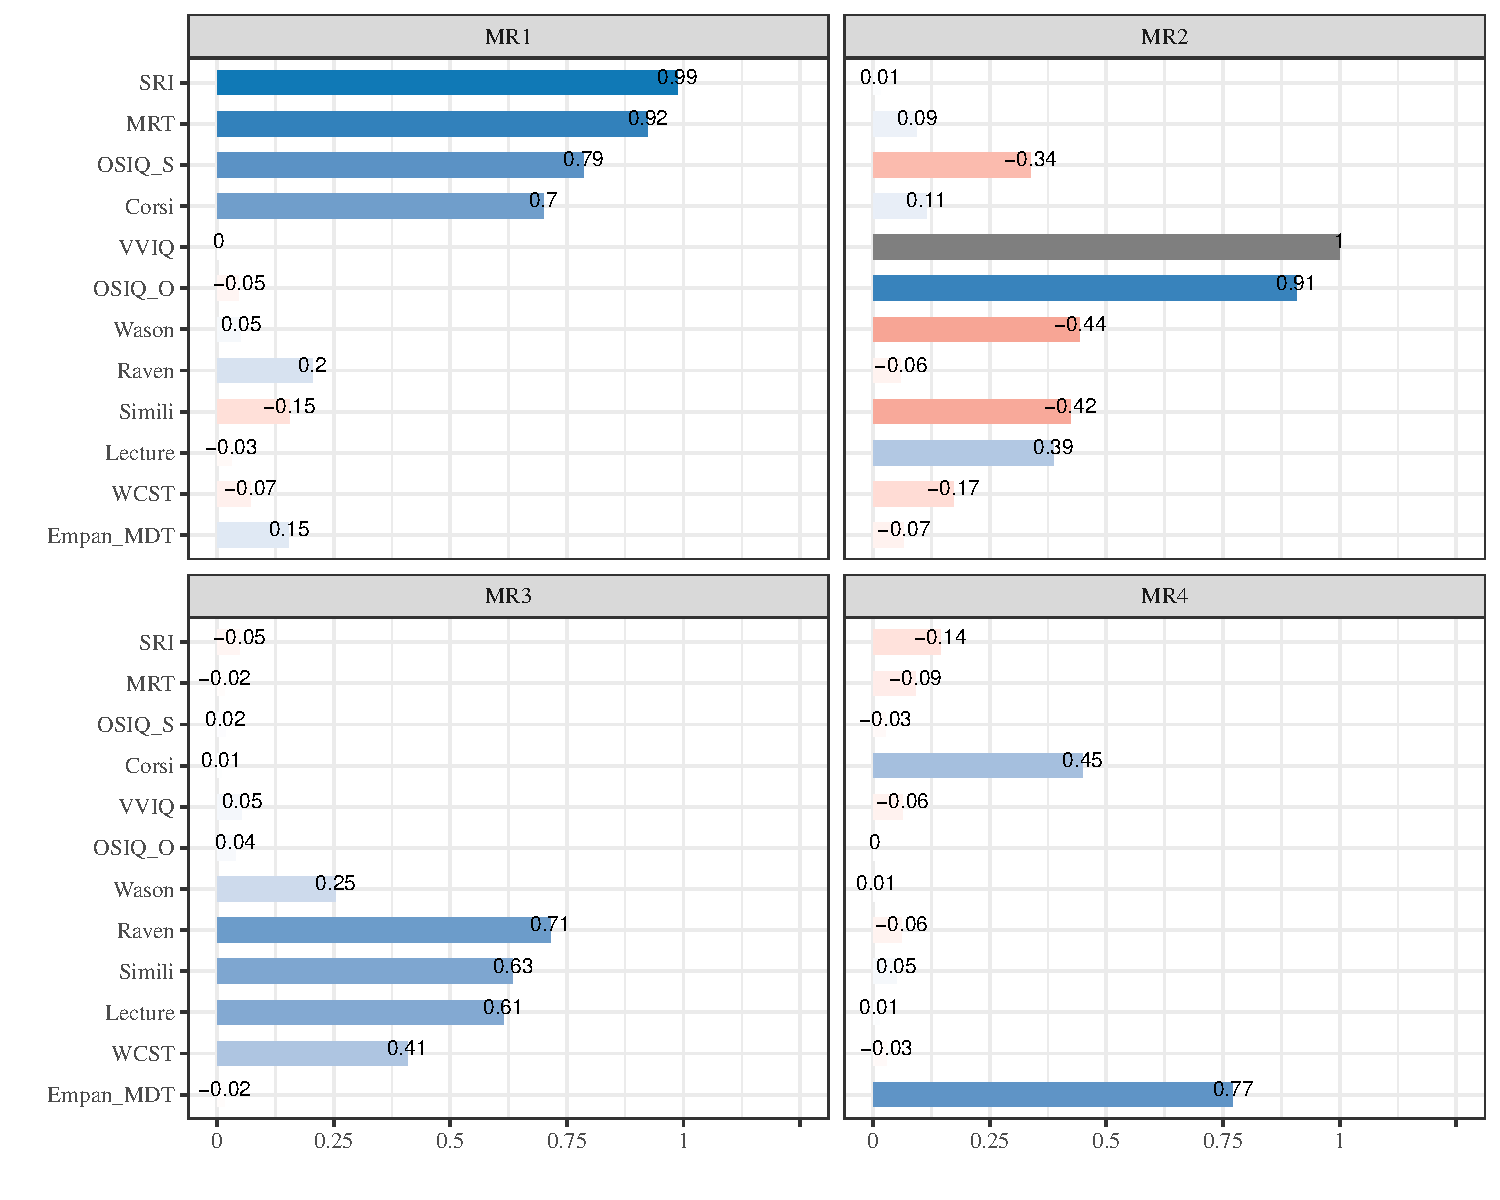
\includegraphics[width=\textwidth,height=0.5\textheight]{simu_0_aphantasia_files/figure-pdf/loadings_graph_annex-1.pdf}

\caption{Poids de chaque variable dans l'Analyse Factorielle Multiple à quatre facteurs.}
\label{loadings_graph_annex}
\end{figure}

\begin{figure}[H]

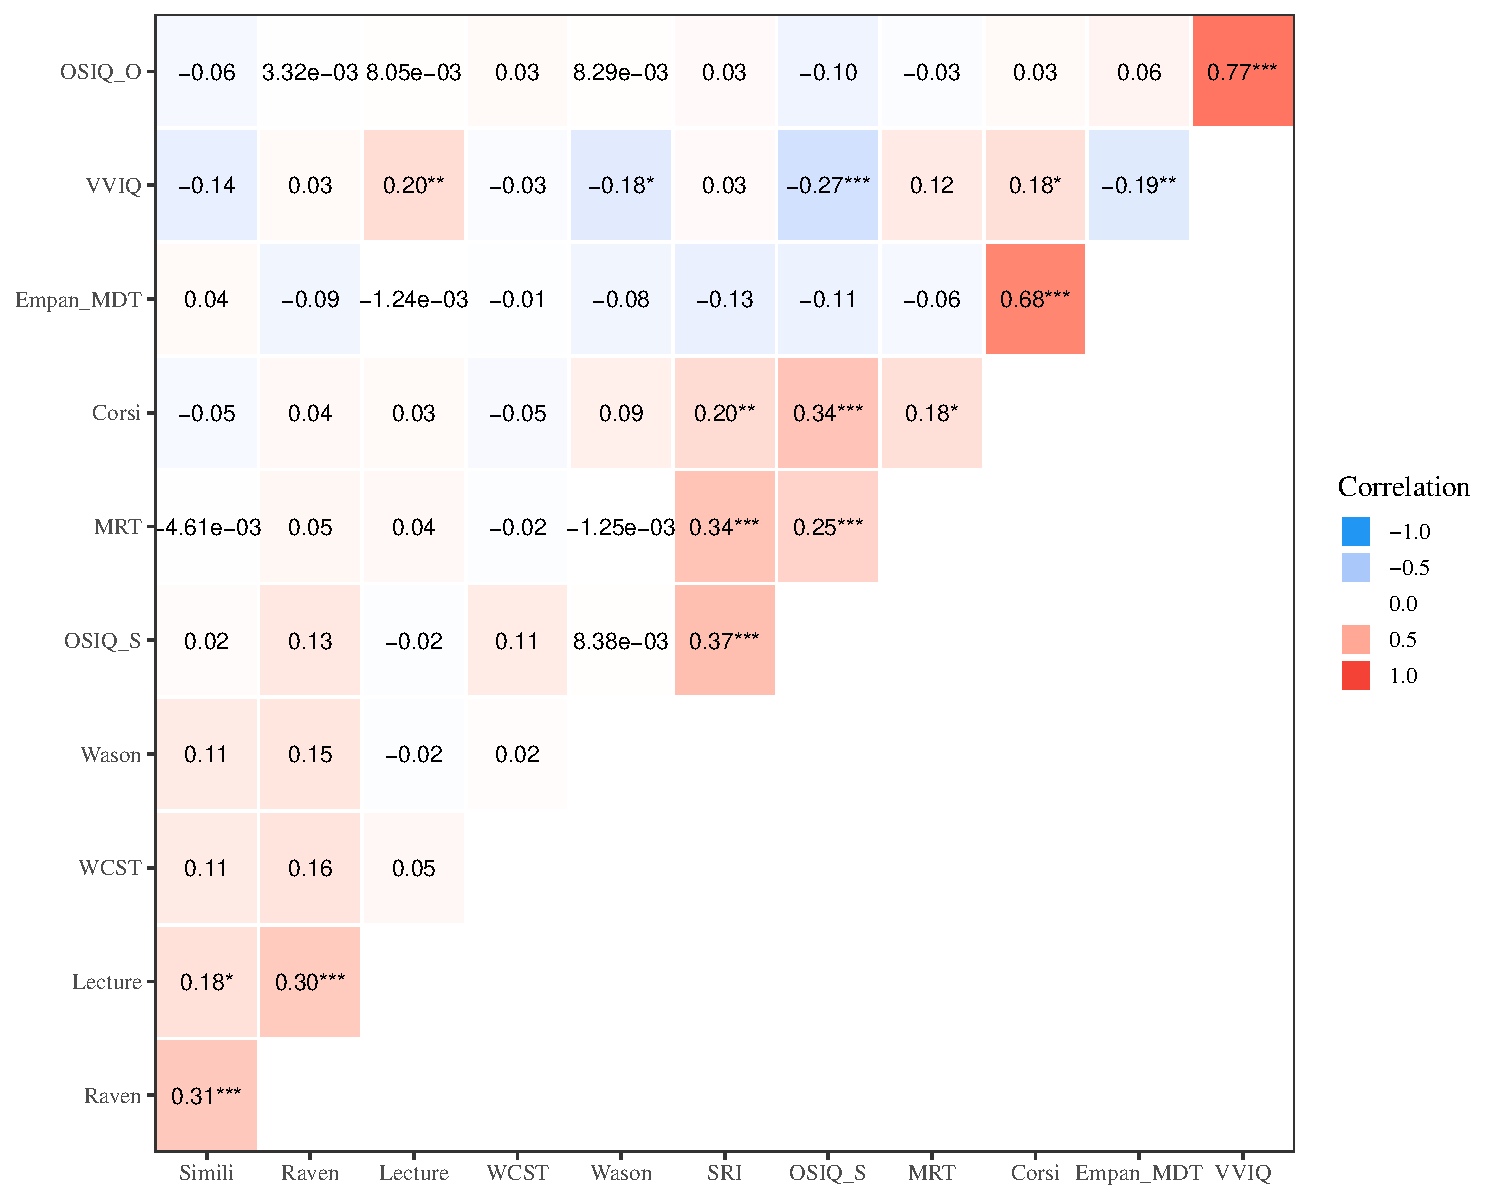
\includegraphics[width=\textwidth,height=0.5\textheight]{simu_0_aphantasia_files/figure-pdf/correlation_matrix-1.pdf}

\caption{Matrice de corrélation entre les toutes les variables mesurées.}
\label{correlation_matrix}
\end{figure}



\end{document}
